\chapter{Testing Quasar Unification: Radiative Transfer In Clumpy Winds}

{\em This chapter is based on the publication:

Matthews J. H., Knigge C., Long K. S., Sim S. A., Higginbottom N., Mangham S. W., 
`Testing quasar unification: radiative transfer in clumpy winds',
2016, MNRAS, 458, 293.}


%%%%%%%%%%%%%%%%%%%%%%%%%%%%%%%%%%%%%%
%
%          INTRODUCTION
%
%%%%%%%%%%%%%%%%%%%%%%%%%%%%%%%%%%%%%%%

\section{Introduction}

In chapters 1 and 2, I reviewed the observational evidence for accretion disc
winds in quasars and luminous AGN, and showed how they may be responsible
for more than just the broad absorption lines and P-Cygni profiles
seen in quasar spectra. In particular, they offer a natural way to
{\em unify} much of the complex phenomenology into one simple picture.

Here, I aim to test that picture using \py, with
the specific aim of determining whether it is possible to 
reproduce the key properties of AGN spectra, including those of BALQSOs, 
using simple kinematic prescriptions for biconical disc winds. 
Past results have been encouraging: H13
produced simulated spectra that resembled those of BALQSOs, as long as 
the luminosity of the X-ray source was relatively low, of order 
\POW{43}{\LUM}, and the mass-loss rate was relatively high, of order the 
mass accretion rate.  However, at higher X-ray luminosities, the wind was
so ionized that UV absorption lines were not produced.  In addition, and 
in part due to limitations inherent in 
the radiative transfer methods, the model failed 
to produce spectra with strong emission lines at any inclination angle.

Here I attempt to address both of these issues, by
allowing for clumping in the outflow and a introducing a more complete
treatment of H and He in the radiative transfer calculations.
Thus, the simulations presented in this chapter treat H and He as full
macro-atoms and metals as simple-atoms, as described extensively
in chapter 3. In order to correctly model the ionizing spectrum for simple-atoms,
I dispense with the dilute blackbody modified-Saha approach and fully solve the ionization
balance using the spectral modelling approach described 
in section~\ref{sec:simple_ionization}. Macro-atoms still have their
ionization and excitation states calculated from MC estimators.

The kinematic model used once again follows the SV93
prescription, and is described, together with the clumping 
implementation, in section~\ref{sec:clumpy_wind_model}.
Section~\ref{sec:qso_results} contains the results obtained from the clumped wind model, 
including comparisons to observational data, as well as some discussion. 
I discuss the results further, and examine their sensitivity to model parameters
and viewing angle in section~\ref{sec:qso_discuss}, which
expands somewhat on the work presented in \cite{M16}.
Finally, I summarise my findings in section~\ref{sec:qso_conclusions}.

%%%%%%%%%%%%%%%%%%%%%%%%%%%%%%%%%%%%%%%%%%%%%%%%%
%
% MODEL DESCRIPTION
%
%%%%%%%%%%%%%%%%%%%%%%%%%%%%%%%%%%%%%%%%%%%%%%%%%

\section{A Clumpy Biconical Disk Wind Model for Quasars}
\label{sec:clumpy_wind_model}
Here, I once again adopt the SV93 kinematic prescription for a 
biconical disc wind model described in section~\ref{sec:sv93_model}
A schematic is shown in Fig.~\ref{fig:cartoon_qso},
with key aspects marked. The general biconical
geometry is similar to that invoked by \cite{MCGV95} and 
\cite{elvis2000} to explain the phenomenonology
of quasars and BALQSOs.

\begin{figure} 
\centering
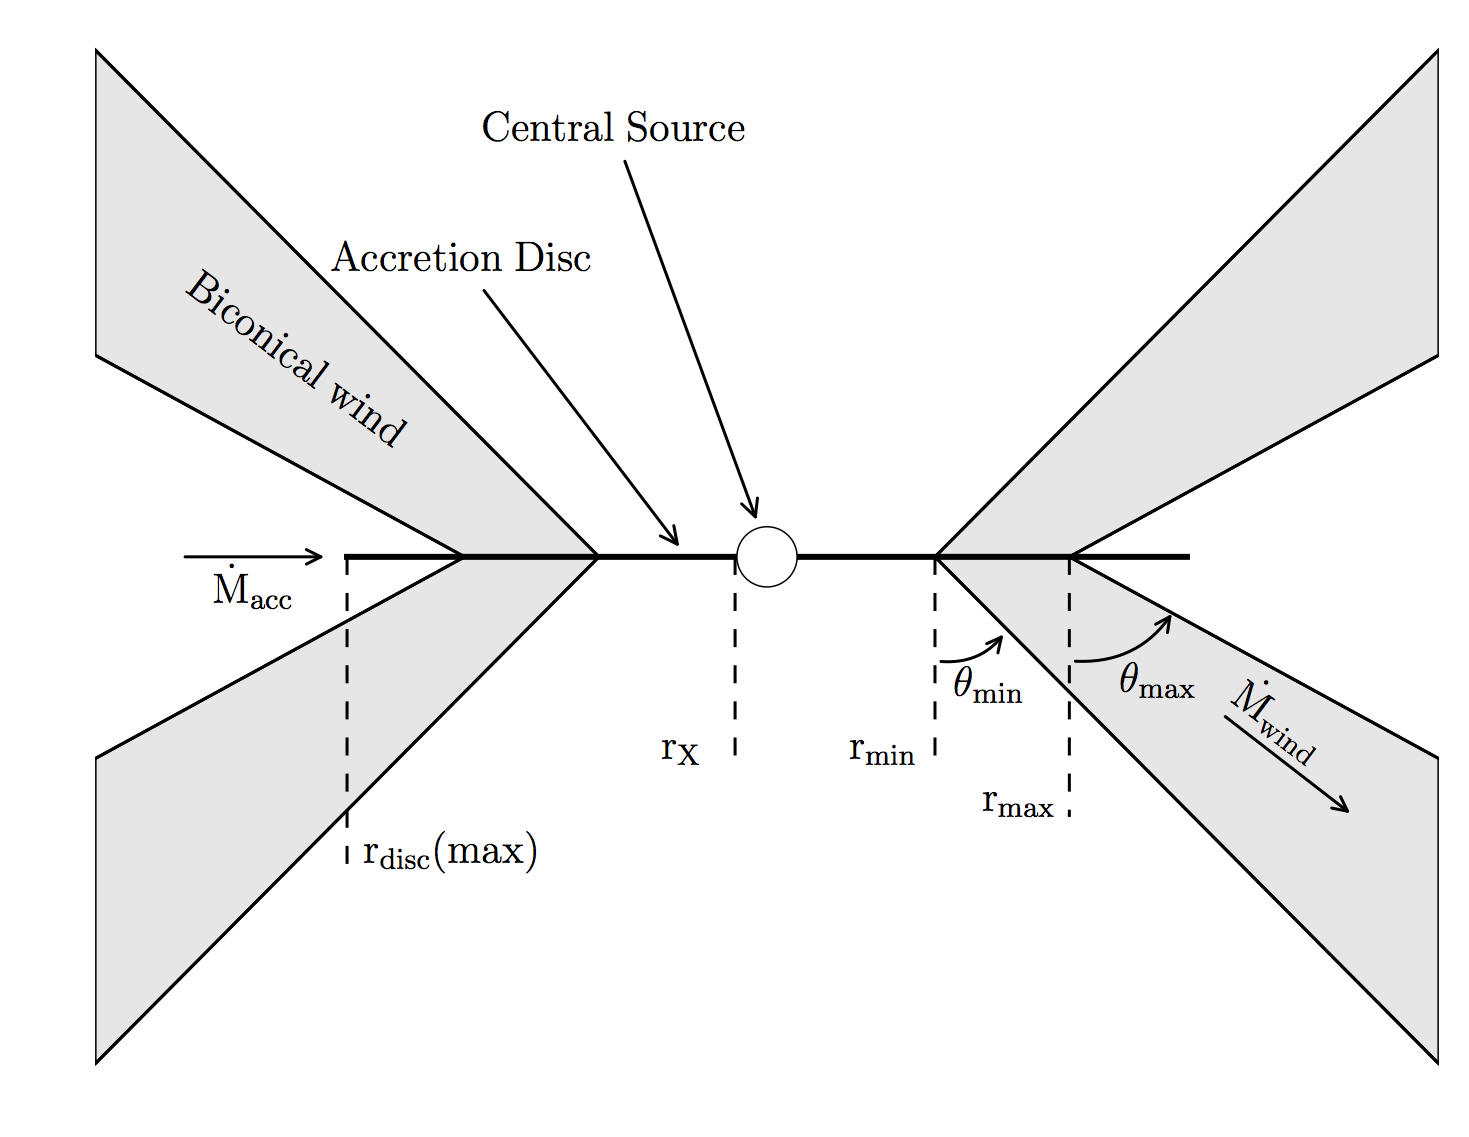
\includegraphics[width=1.0\textwidth]{figures/06-agnpaper/fig1.png}
\caption
[A cartoon showing the geometry and some key parameters of
the biconical quasar wind model.]
{
A cartoon showing the geometry and some key parameters of
the biconical quasar wind model.
}
\label{fig:cartoon_qso}
\end{figure} 

\subsection{Photon Sources}
\label{sec:photon_sources}

Two sources of r-packets are included in the model:
An accretion disc and a central X-ray s ce.
The accretion disc is assumed to be geometrically thin, 
but optically thick.
Accordingly, the disc is modelled as an ensemble of blackbodies with a 
\cite{shakurasunyaev1973} effective temperature profile. 
The emergent SED is then determined by the specified accretion rate ($\dot{M}$)
and central BH mass ($M_{BH}$).
All photon sources in the model are opaque, meaning
that r-packets that strike them are destroyed.
The inner radius of the disc extends to the innermost 
stable circular orbit (ISCO) of the BH. 
I assume a Schwarzchild BH with an ISCO at $6~r_G$, where 
$r_G = GM_{BH}/c^2$ is the gravitational radius.
For a $10^9~M_\odot$ BH, this is equal to $8.85\times10^{14}~{\rm cm}$ 
or $\sim10^{-4}~{\rm pc}$.  


The X-ray source is treated as an isotropic sphere at the ISCO,
which emits $r$-packets according to a power law in flux with index $\alpha_X$, of the form
\begin{equation}
F_X (\nu) = K_X \nu^{\alpha_X}.
\end{equation}
The normalisation, $K_X$ of this power law is such that it 
produces the specified 2-10~keV luminosity, $L_X$.
The input spectrum for the simulations is therefore a simple combination
of a power law X-ray component and accretion disc spectrum; an example input
spectrum is shown in Fig.~\ref{fig:qso_model_sed}. In actual fact, this
spectrum will be angle dependent due to the geometry of the system and 
the angular emissivity profile of the accretion disc (see sections~\ref{sec:xray}
and \ref{sec:ew_in_model}.
Photons, or $r$-packets, produced by the accretion disc and central X-ray source
are reprocessed by the wind. This reprocessing is dealt with by enforcing strict
radiative equilibrium ({\em modulo} adiabatic cooling; see section~\ref{sec:estimators})
via the indivisible energy packet constraint.  

\begin{figure} 
\centering
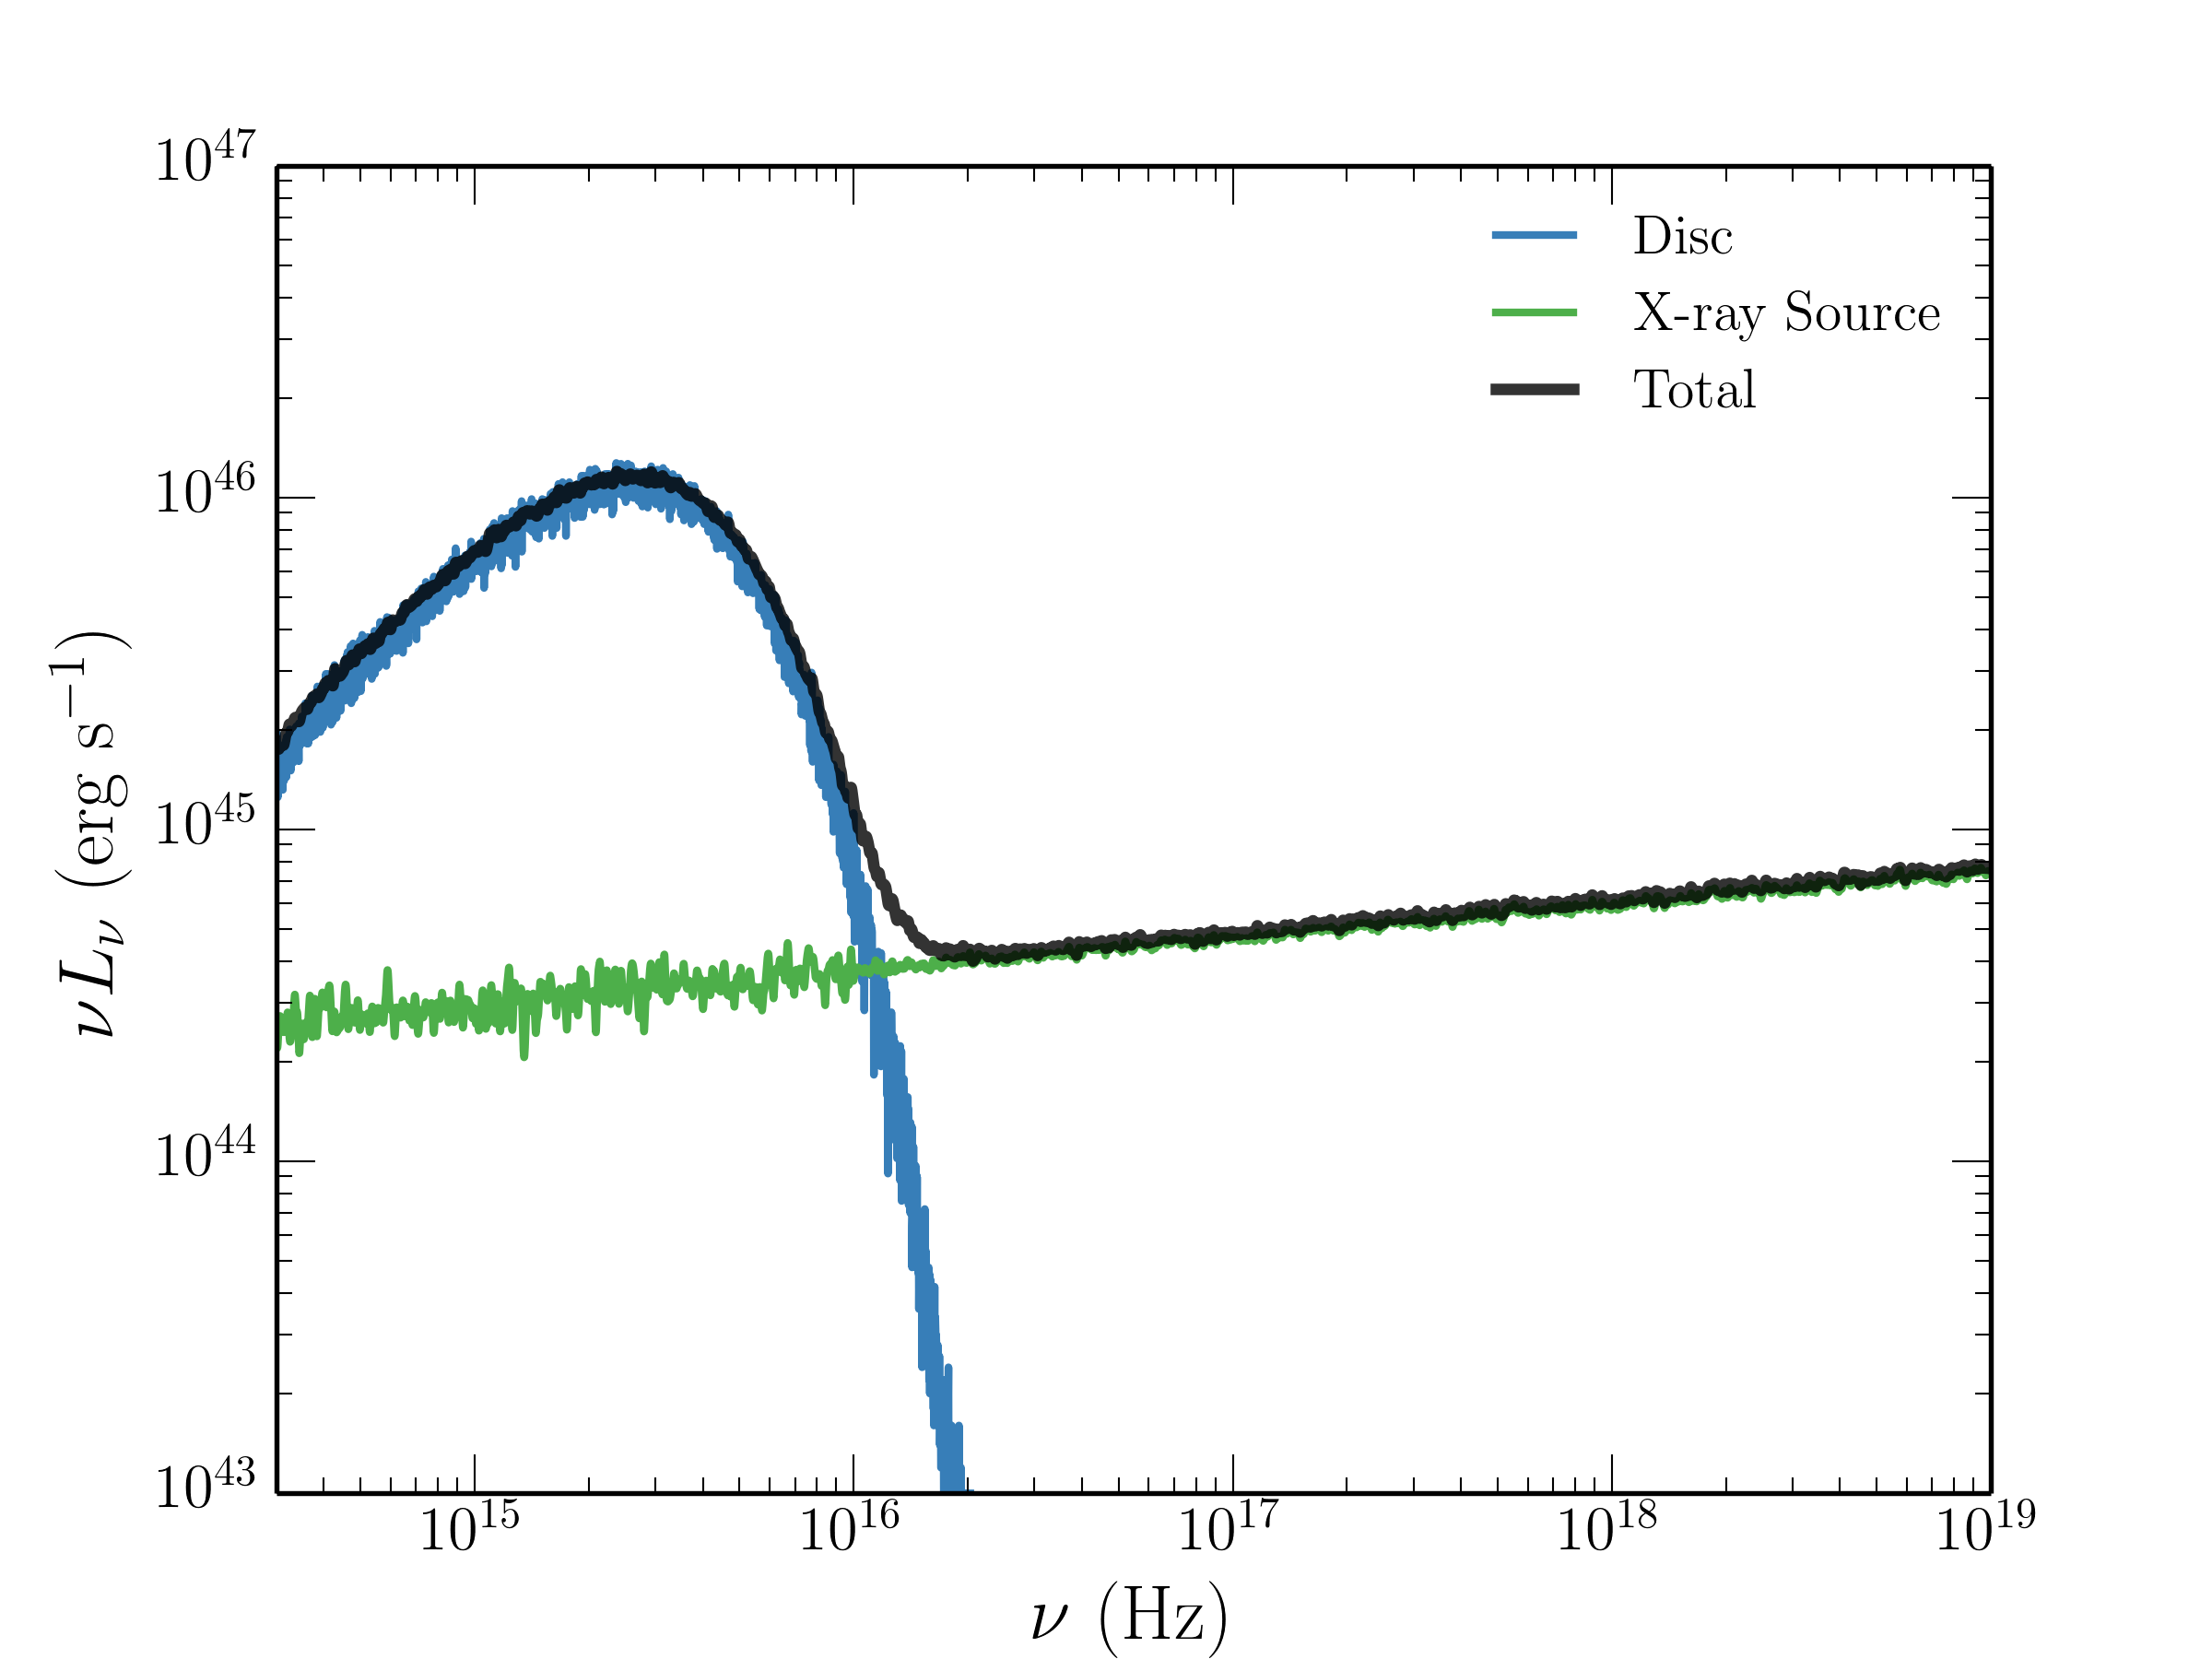
\includegraphics[width=1.0\textwidth]{figures/06-agnpaper/qso_model_sed.png}
\caption
[The input spectrum used for the quasar modelling.]
{
The input spectrum used for the quasar modelling.
}
\label{fig:qso_model_sed}
\end{figure} 

\subsection{A Simple Approximation for Clumping}

In previous modelling efforts with \py, a smooth outflow was assumed, 
such that the density at a given point was determined only by the 
kinematic parameters and mass loss rate. However, as already discussed,
AGN winds exhibit significant substructure -- the outflow is expected to be
{\em clumpy}, rather than smooth, and probably on a variety of scales. 
A clumpy outflow offers a possible solution to the so-called `over-ionization problem' in 
quasar and AGN outflows \citep[e.g.][]{junk1983,weymann1985,hamann2013}. 
This is the main motivation for incorporating clumping into the model.

Deciding on how to implement clumping into the existing wind models was not straightforward.
First, and most importantly, the physical scale lengths and density contrasts in AGN outflows are not well-constrained from observations or theory.  As a result, while one could envision in principle, clouds with a variety of sizes and density contrasts varying perhaps as function of radius, there would have been very little guidance on how to set nominal values of the various parameters of such a model.
Second, there are significant computational difficulties associated with adequately resolving and realistically modelling a series of small scale, high density regions with a MCRT
-- or for that matter, a hydrodynamical -- code. 
Given the lack of knowledge about the actual type of clumping, I have implemented
a simple approximation used successfully in stellar wind modelling, known as 
{\em microclumping} \citep[e.g.][]{hamann1998,hilliermiller1999,hamann2008}.  

The underlying assumption of microclumping is that clump sizes 
are much smaller than the 
typical photon mean free path, and thus the clumps are 
both geometrically and optically thin. This approach 
allows one to treat clumps only in terms of their volume filling factor, $f_V$, 
instead of having to specify separately their size and density distributions.
In this model, $f_V$ is independent of position.
The inter-clump medium is modeled as a vacuum,
although the outflow is still non-porous and axisymmetric.
This approach therefore assumes that the inter-clump medium
is unimportant in determing the output spectrum, which
is expected to be true only when density constrasts are large and
the inter-clump medium is both very ionized and of low emissivity and opacity.
The density of the clumps is multiplied by the ``density enhancement'' 
$D=1/f_V$. Opacities, $\kappa$, and emissivities, $j$, 
can then be expressed as 
\begin{equation}
\kappa = f_V \kappa_C(D);~~j = f_V j_C(D).
\end{equation}
Here the subscript $C$ denotes that the quantity is calculated using the 
enhanced density in the clump. The resultant effect is that, {\em for fixed temperature},
processes that are linear in density, such as electron scattering, are unchanged, 
as $f_V$ and $D$ will cancel out. However, any quantity that scales with the square of density, 
such as collisional excitation or recombination, will increase by a factor of $D$.
In \py, the temperature is not fixed, and is instead set by balancing heating and 
cooling in a given cell. In the presence of an X-ray source, this thermal balance is 
generally dominated by bound-free heating and line cooling. The main effect of including 
clumping in this modelling is that it moderates the ionization state due to the increased 
density. This allows an increase in the ionizing luminosity, amplifying the amount of
bound-free heating and also increasing the competing line cooling term
(thermal line emission).

The shortest length scale in a Sobolev MCRT treatment such as that used here
is normally the Sobolev length, given by
\begin{equation}
l_S = \frac{v_{th}}{| dv/ds |}
\end{equation}
This is typically $\sim10^{13}$~cm near the disc plane, increasing outwards.
The Sobolev length calculated from the mean velocity gradient in a cell
is shown, together with the size of the cell
and Thomson mean free path, in Fig.~\ref{fig:length_scales}.
The mean density is used to calculate the Sobolev optical depth, 
which assumes that $l_S$ is greater than the typical clump size.
Thus for the microclumping assumption to be formally correct, 
clumps should be no larger than $\sim10^{12}$~cm.
This size scale is not unreasonable for quasar outflows, as
\cite{dekool1995} suggest that BAL flows may have low filling factors with
clump sizes of $\sim10^{11}$~cm.
% An additional concern with this approach to clumping is that the clumps
% may rapidly cool and expand into the inter-clump medium. This is a well-known
% issue in BLR and outflow models (REFs), and requires some kind of confining mechanism,
% such as magnetic confinement \cite[e.g.][]{dekool1995}. Alternatively, as already discussed,
% the LDI may cause clumpy flows as expected in stellar winds.}
\begin{figure} 
\centering
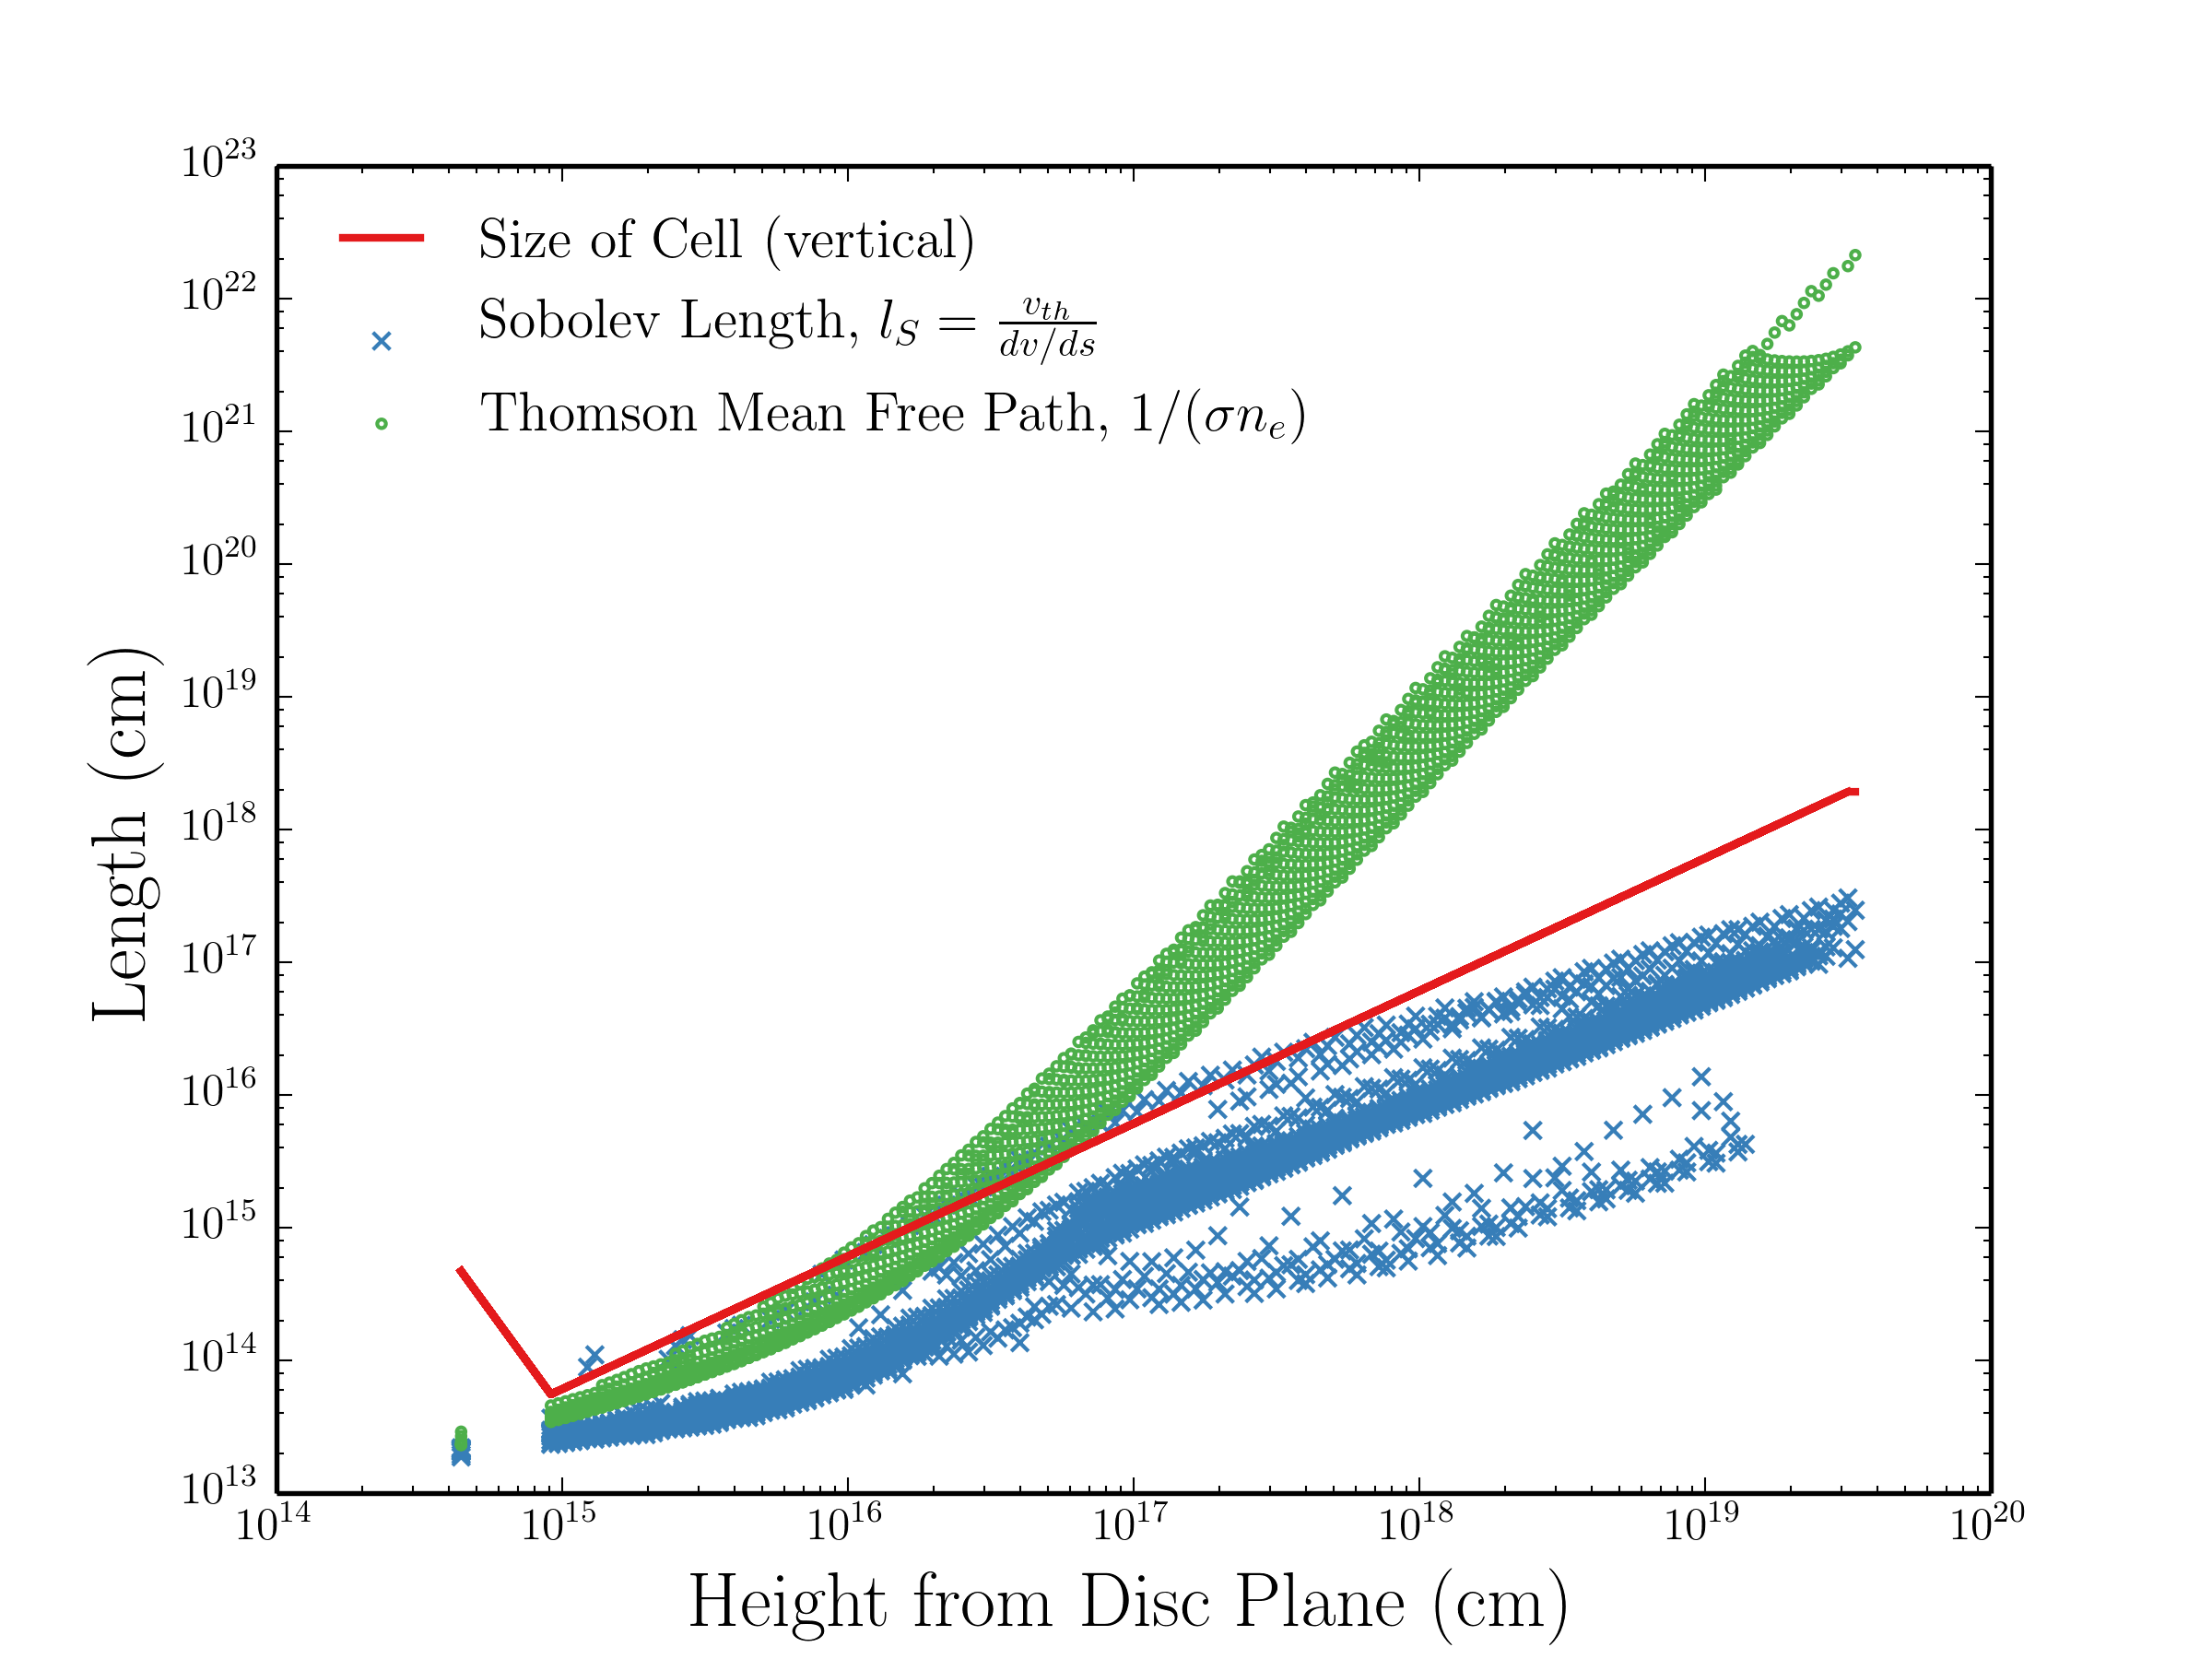
\includegraphics[width=1.0\textwidth]{figures/06-agnpaper/size_of_clumps.png}
\caption
[Some typical length scales for the fiducial model.]
{
Some typical length scales for the fiducial model. 
This places a formal limit of $\sim10^{12}$~cm on clump sizes 
in the microclumping framework, and confirms that the cells are sufficiently
larger than the Sobolev length in almost all cases.
}
\label{fig:length_scales}
\end{figure} 

This clumping treatment is necessarily simple; it does not adequately
represent the complex substructures and stratifications in ionization
state expected in AGN outflows. 
Nevertheless, this parameterization 
allows simple estimates of the effect clumping has on the ionization 
state and emergent line emission.


\subsection{The Simulation Grid}
\label{sec:sim_grid}
Using this prescription, I conducted a limited parameter
search over a 5-dimensional parameter space involving the 
variables $r_{\mathrm{min}}$, $\theta_{\mathrm{min}}$, $f_V$, $\alpha$ and $R_v$.
The grid points are shown in table~\ref{grid_table}.
The aim here was to first fix $M_{BH}$ and $\dot{M}$ to their H13 values,
and increase $L_X$ to $10^{45}$~erg~s$^{-1}$ (a more realistic value for a 
quasar of $10^9~M_\odot$ and an Eddington fraction of $0.2$; see section~\ref{sec:xray}).

These models were then evaluated based on 
how closely their synthetic spectra reproduced the 
following properties of quasars and BALQSOs:

\begin{itemize}
\item UV absorption lines 
with $BI > 0$ at $\sim20\%$ of viewing angles \cite[e.g.][]{knigge2008};
\item Line emission emerging at low inclinations, with $\mathrm{EW}\sim40$~\AA\ in \civline\ \citep[e.g. ][]{shen2011};
\item H recombination lines with $EW\sim50$~\AA\ in \la\ \citep[e.g. ][]{shen2011};
\item  \mg\ and \al\ (LoBAL) absorption features with $BI > 0$ at a subset of 
BAL viewing angles;
\item Verisimilitude with quasar composite spectra.
\end{itemize}
Here $BI$ is the `Balnicity Index' (Weymann et al. 1991), given by
\begin{equation}
BI = \int^{25000~{\rm km~s}^{-1}}_{3000~{\rm km~s}^{-1}} C \left( 1 - \frac{f(v)}{0.9} \right) dv.
\end{equation}
The constant $C=0$ everywhere, unless the normalized flux
has satisfied $f(v)<0.9$ continuously for at least $2000$~km~s$^{−1}$, 
whereby $C$ is set to $1$.

In the next section, I present one of the most promising models,
which I refer to as the fiducial model, and discuss
the various successes and failures with respect to the above criteria.
This allows insight into fundamental geometrical 
and physical constraints to be gained, 
and the potential for unification assessed. 
I then discuss the sensitivity to key parameters in section~\ref{sec:param_sens}.
The full grid, including output synthetic spectra and plots can be found at
\url{jhmatthews.github.io/quasar-wind-grid/}.

\begin{table}
\centering
\begin{tabular}{p{2cm}p{1cm}p{1cm}p{1cm}p{1cm}}
Parameter & \multicolumn{4}{l}{Grid Point Values}  \\
\hline \hline 
$r_{\mathrm{min}}$ 	&	 $60r_{g}$ & $180r_{g}$ & \multicolumn{2}{l}{$300r_{g}$} \\ 
$\theta_{\mathrm{min}}$ 	& $55^{\circ}$ & \multicolumn{3}{l}{$70^{\circ}$} \\ 
$R_v$  	        &	 $10^{18}$~cm & \multicolumn{3}{l}{$10^{19}$~cm} \\ 
$\alpha$ 	&	 $0.5$ & $0.6$ & $0.75$ & $1.5$ \\
$f_V$ 	&	 $0.01$ & \multicolumn{3}{l}{$0.1$}  \\
\hline 
\end{tabular}
\caption
[The grid points used in the parameter search for quasar wind models]
{The grid points used in the parameter search.
The sensitivity to some of these parameters is discussed 
further in section~\ref{sec:param_sens}}
\label{grid_table}
\end{table}



%%%%%%%%%%%%%%%%%%%%%%%%%%%%%%%%%%%%%%%%%%%%%%%%%

% RESULTS

%%%%%%%%%%%%%%%%%%%%%%%%%%%%%%%%%%%%%%%%%%%%%%%%%


\section{Results and Analysis from a Fiducial Model}
\label{sec:qso_results}
Here I describe the results from a fiducial model,
and discuss these results in the context of the criteria 
presented in section~\ref{sec:sim_grid}. 
The parameters of this model are shown in table~\ref{wind_param}.
Parameters differing from the benchmark model of H13 are 
highlighted with an asterisk. In this section, I examine the physical 
conditions of the flow, and present the synthetic spectra, before comparing
the X-ray properties of this particular model to samples of
quasars and luminous AGN. 

\begin{table}
\centering
\begin{tabular}{p{3cm}p{4cm}}
\hline Parameter 	&	 Value \\ 
\hline \hline 
$M_{BH}$ 	 &	 $1\times 10^9~\rm{M_{\odot}}$ \\ 
$\dot{M}_{\mathrm{acc}}$ 	 &	 $5~M_{\odot}\mathrm{yr}^{-1} \simeq 0.2~\dot{M}_{\mathrm{Edd}}$\\ 
$\alpha_X$ 	 &	 $-0.9$ \\ 
$L_{X} $ 	 &	 $10^{45}~\rm{erg~s^{-1}}$$^*$ \\ 
$r_{\mathrm{disc}}(\mathrm{min})=r_{X}$   &	 $6r_g=8.8\times10^{14}~{\rm cm}$ \\ 
$r_{\mathrm{disc}}(\mathrm{max})$   &	 $3400r_g = 5\times10^{17}~{\rm cm}$ \\ 
$\dot{M}_W$  &	 $5~M_{\odot}yr^{-1}$ \\ 
$r_{\mathrm{min}}$ 	&	 $300r_{g} = 4.4\times10^{16}~{\rm cm}$\\ 
$r_{\mathrm{max}}$ 	&	 $600r_{g} = 8.8\times10^{16}~{\rm cm}$ \\ 
$\theta_{\mathrm{min}}$ 	&	 $70.0^{\circ}$ \\ 
$\theta_{\mathrm{max}}$ 	&	 $82.0^{\circ}$ \\ 
%%$\lambda$ 	&	 $0$ \\ 
$v_{\infty}(r_0)$ 	&	 $v_{\mathrm{esc}}(r_0)$ \\ 
$R_v$  	        &	 $10^{19}$~cm$^*$ \\ 
$\alpha$ 	&	 $0.5^*$ \\
$f_V$ 	&	 $0.01^*$  \\
$n_x$ 	&	 $100$  \\
$n_z$ 	&	 $200$  \\
\hline 
\end{tabular}
\caption
[Model parameters for the fiducial quasar model.]
{Wind geometry parameters 
used in the fiducial model, as defined in the text and Fig.~\ref{fig:cartoon_qso}.
Parameters differing from the benchmark model of H13 are 
highlighted with an asterisk.}
\label{wind_param}
\end{table}



\subsection{Physical Conditions and Ionization State}


\begin{figure*}
\centering
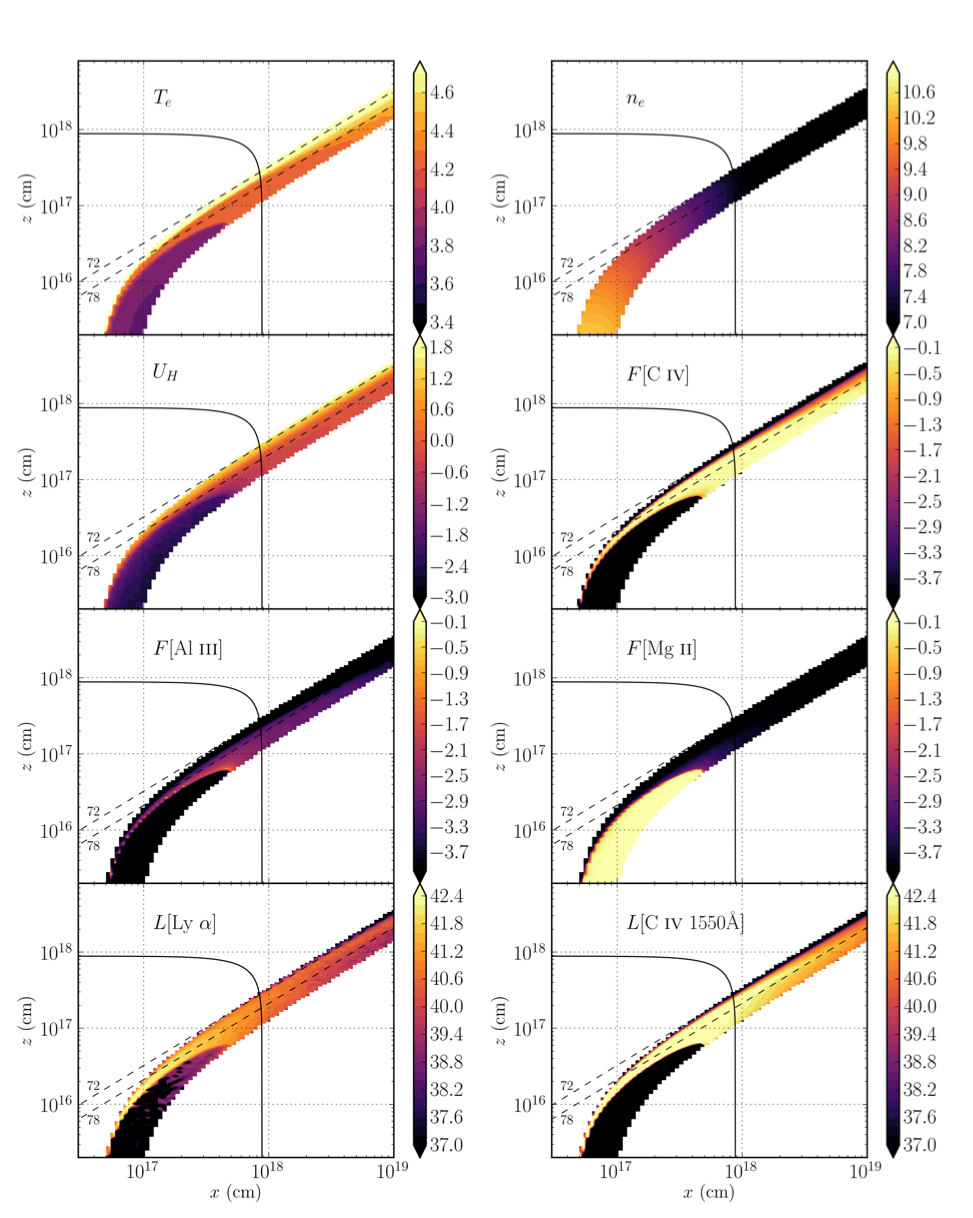
\includegraphics[width=1.0\textwidth]{figures/06-agnpaper/fig2.png}
\caption
[Contour plots showing the logarithm of some important 
physical properties of the quasar outflow.]
{
Contour plots showing the logarithm of some important 
physical properties of the outflow. The spatial scales are
logarithmic and the $x$ and $z$ scales are not the same.
Symbols are defined in the text.
The solid black line marks a sphere at $1000~r_G$.
The dotted lines show the $72^\circ$ and $78^\circ$ sightlines 
to the centre of the system, and illustrate that different sightlines
intersect material of different ionization states.
The line luminosities, $L$, represent the luminosity of photons
escaping the Sobolev region for each line. These photons do not
necessarily escape to infinity.
}
\label{fig:wind}
\end{figure*}

\begin{figure} 
\centering
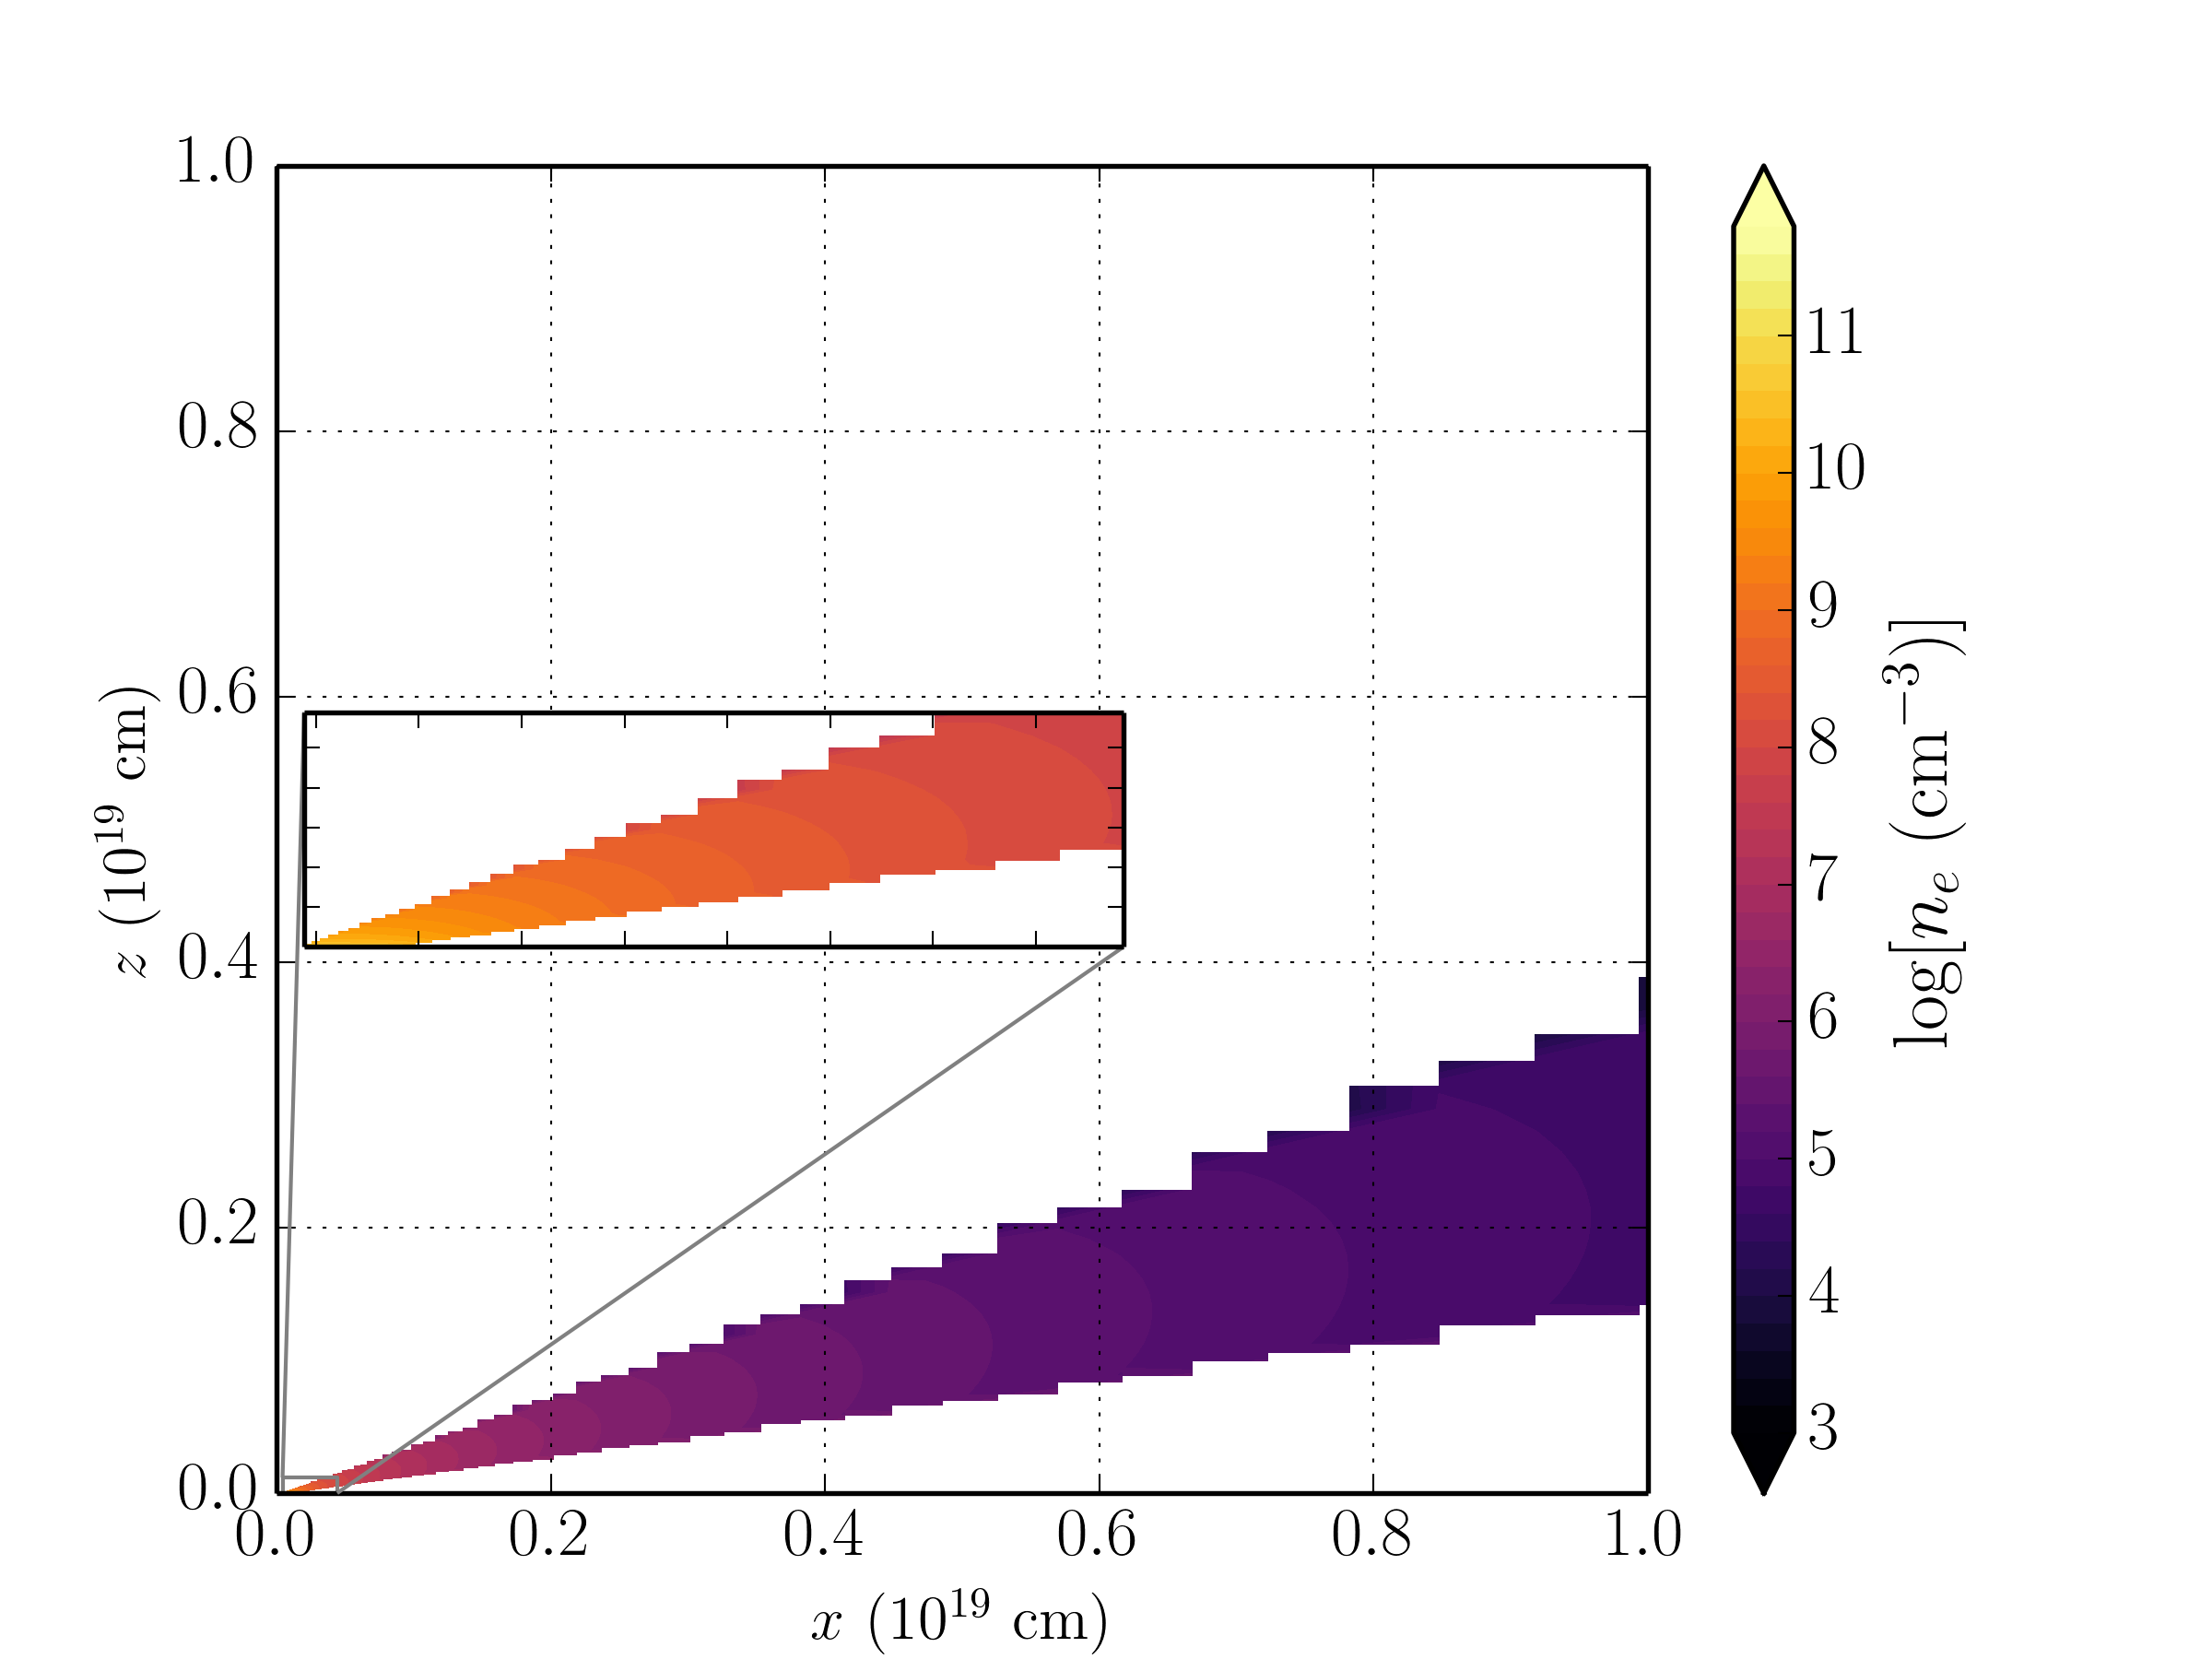
\includegraphics[width=0.8\textwidth]{figures/06-agnpaper/ne_in_wind.png}
\caption
[The electron density in the fiducial model on linear axes.]
{
The electron density in the model, this time on linear axes
in order to illustrate the density contrasts and scale of the system.
The plot is on the scale of the acceleration length, whereas
the inset is a box of $2700 \times 800 r_G$, where the bottom left corner
corresponds to the base of the innermost streamline.
}
\label{fig:ne_in_wind}
\end{figure} 

\noindent
Fig.~\ref{fig:wind} shows the physical properties of the wind.
The wind rises slowly from the disc at first, with densities within clumps
of $n_H \sim 10^{11}~\rm{cm^{-3}}$ close to the disc plane, 
where $n_H$ is the local number density of H. To illustrate the degree
of scale and density ranges in the model I also show $n_e$ in the wind
on a linear scale in Fig.~\ref{fig:ne_in_wind}.
The flow then accelerates over a scale length of $R_V=10^{19}~\rm{cm}$
up to a terminal velocity equal to the escape velocity at the streamline base
($\sim10,000~\rm{km~s^{-1}}$). This gradual acceleration results in
a wind that exhibits a stratified ionization structure, with low ionization material
in the base of the wind giving way to highly ionized plasma further out.
This is illustrated in Fig.~\ref{fig:wind} 
by the panels showing the ion fraction $F=n_j/n_{tot}$ of some important ions.
The clumped wind produces the range of ionization states observed
in quasars and BALQSOs, while adopting a realistic $2-10$ keV X-ray luminosity
of $L_{X}=10^{45}~\rm{erg~s^{-1}}$. Without clumping, this wind would be over-ionized 
to the extent that opacities in e.g., \civ\ would be entirely negligible (see H13).

One common way to quantify the ionization state of a plasma
is through the ionization parameter, $U_H$, given by equation~\ref{eq:ip}.
Shown in Fig.~\ref{fig:wind},
the ionization parameter is a useful measure of the global ionization state,
as it represents the ratio of the number density of 
H ionizing photons to the local H density.
It is, however, a poor representation of the 
ionization state of species such as \civ\ as it encodes no information
about the shape of the SED. In this case, the X-ray photons 
are dominant in the photoionization of the UV resonance line ions. 
This explains why a factor of 100 increase in X-ray luminosity requires
a clumping factor of 0.01, even though the value of $U_H$ decreases by only a factor of $\sim10$ compared to H13. 

The total line luminosity also increases dramatically compared to the unclumped model
described by H13. This is because the denser outflow can absorb the increased
X-ray luminosity without becoming over-ionized, leading to a hot plasma which
produces strong collisionally excited line emission.
This line emission typically emerges on the edge of the wind
nearest the central source. The location of the line emitting regions
is dependent on the ionization state, as well as the incident X-rays.
The radii of these emitting regions is important,
and can be compared to observations. The line luminosities, $L$,
shown in the figure correspond to the luminosity in $\LUM$ of photons
escaping the Sobolev region for each line. 
As shown in Fig.~\ref{fig:wind},
the \civline\ line in the fiducial model is typically formed between 
$100-1000~r_G$ ($\sim10^{17}-10^{18}~\rm{cm}$).
This is in rough agreement with the reverberation mapping 
results of \cite{kaspi2007} 
for the $2.6\times10^{9} M_\odot$ quasar S5 0836+71,
and also compares favourably with microlensing measurements of the size of the
\civline\ emission line region in the BALQSO H1413+117 \citep{odowd2015}.


\subsection{Synthetic Spectra: Comparison to Observations}

\begin{figure*}
\centering
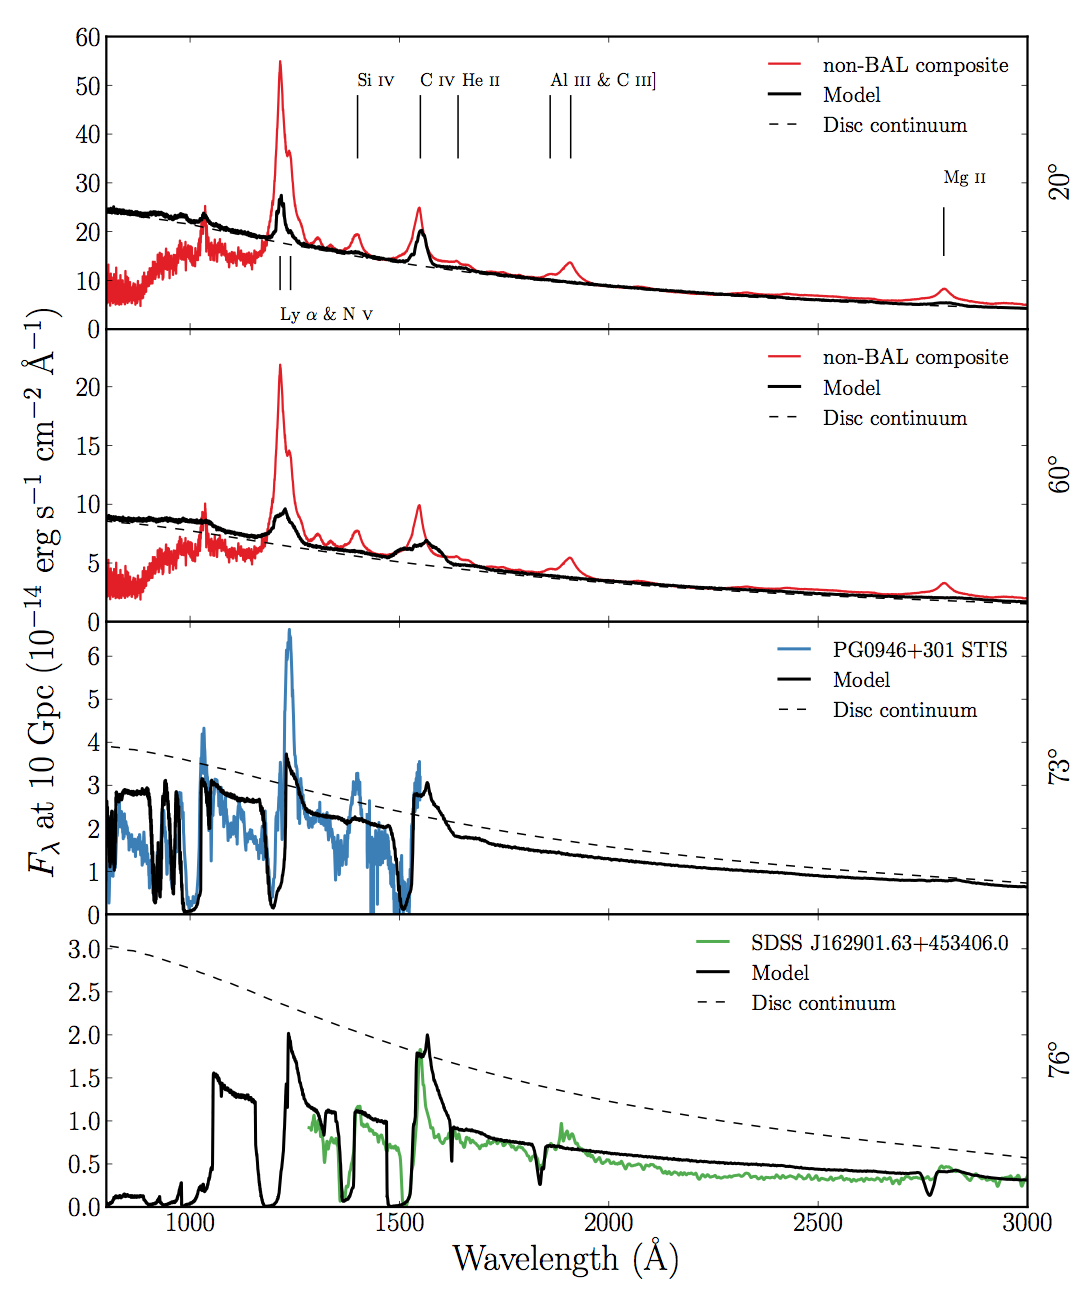
\includegraphics[width=1.0\textwidth]{figures/06-agnpaper/fig3.png}
\caption
[Synthetic spectra at four viewing angles for the fiducial quasar model.]
{
Synthetic spectra at four viewing angles for the fiducial model. At 
$20^\circ$ and $60^\circ$ I show a comparison to an SDSS quasar composite
from Reichard et al. (2003). At $73^\circ$ and $76^\circ$ I show a comparison to
an {\sl HST} STIS spectrum of the high BALnicity BALQSO 
PG0946+301 (Arav et al. 2000), and an SDSS spectrum of the LoBAL quasar 
SDSS J162901.63+453406.0, respectively. The dotted line shows a disc
only continuum to show the effect of the outflow on the continuum level. 
All the spectra are scaled to the model flux at $2000$~\AA, expect for the 
{\sl HST} STIS spectrum of PG0946+301, which is scaled to $1350$~\AA\
due to the incomplete wavelength coverage.
% HST STIS spectrum of PG0946+301 (Arav et al. 2000)
}
\label{fig:uvspec}
\end{figure*}

\begin{figure} 
\centering
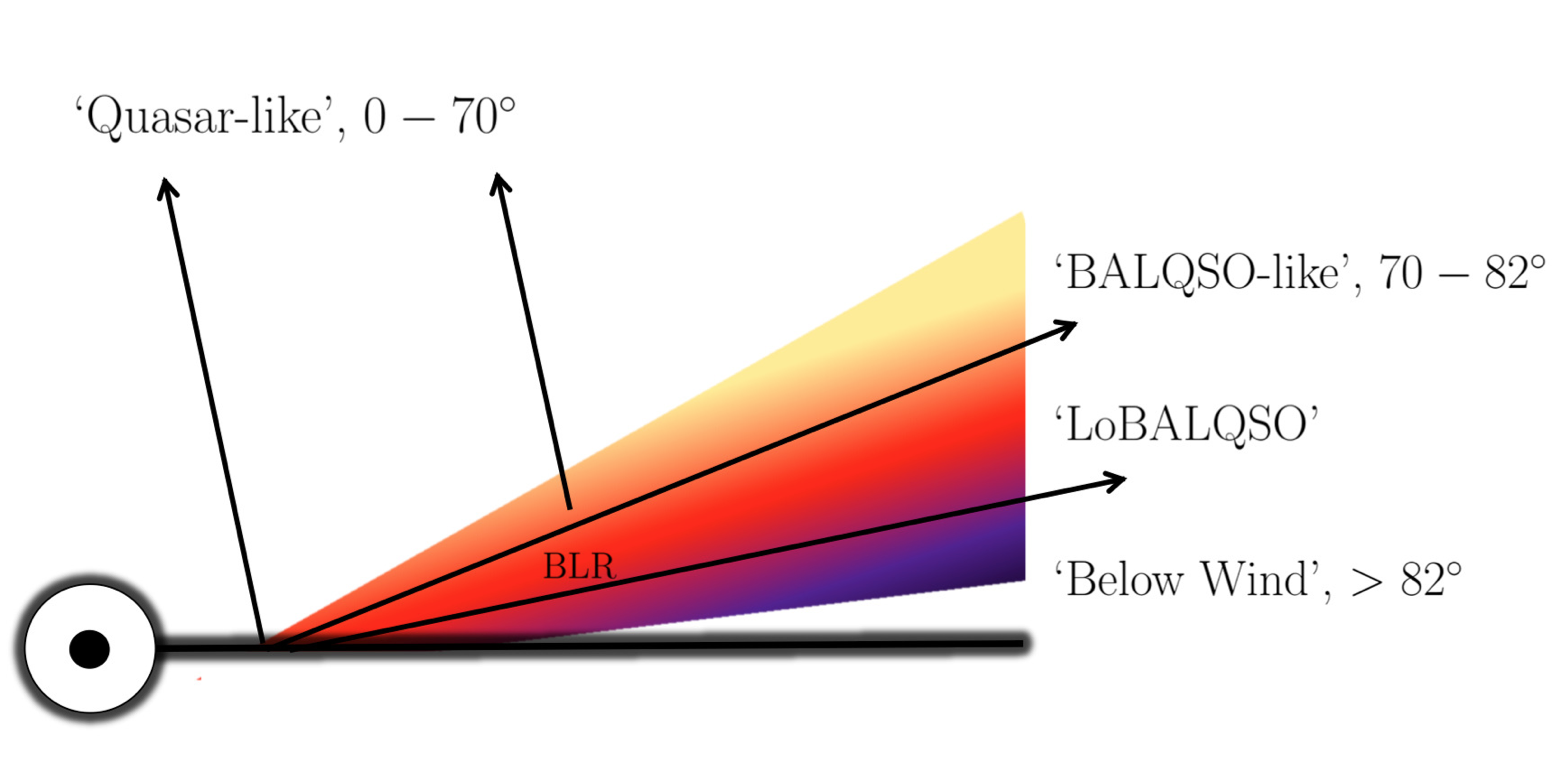
\includegraphics[width=1.0\textwidth]{figures/06-agnpaper/fig4.png}
\caption
[A schematic showing the broad classes of sightline 
in the fiducial model.]
{
A cartoon describing the broad classes of sightline 
in the fiducial model, illustrating how geometric effects lead to 
the different emergent spectra. The colour gradient is approximate,
but indicates the stratified ionization structure, 
from highly ionized (yellow) to low ionization (purple) material.
%[FIGURE NEEDS IMPROVING]
}
\label{fig:sightline}
\end{figure} 

\begin{figure*}
\centering
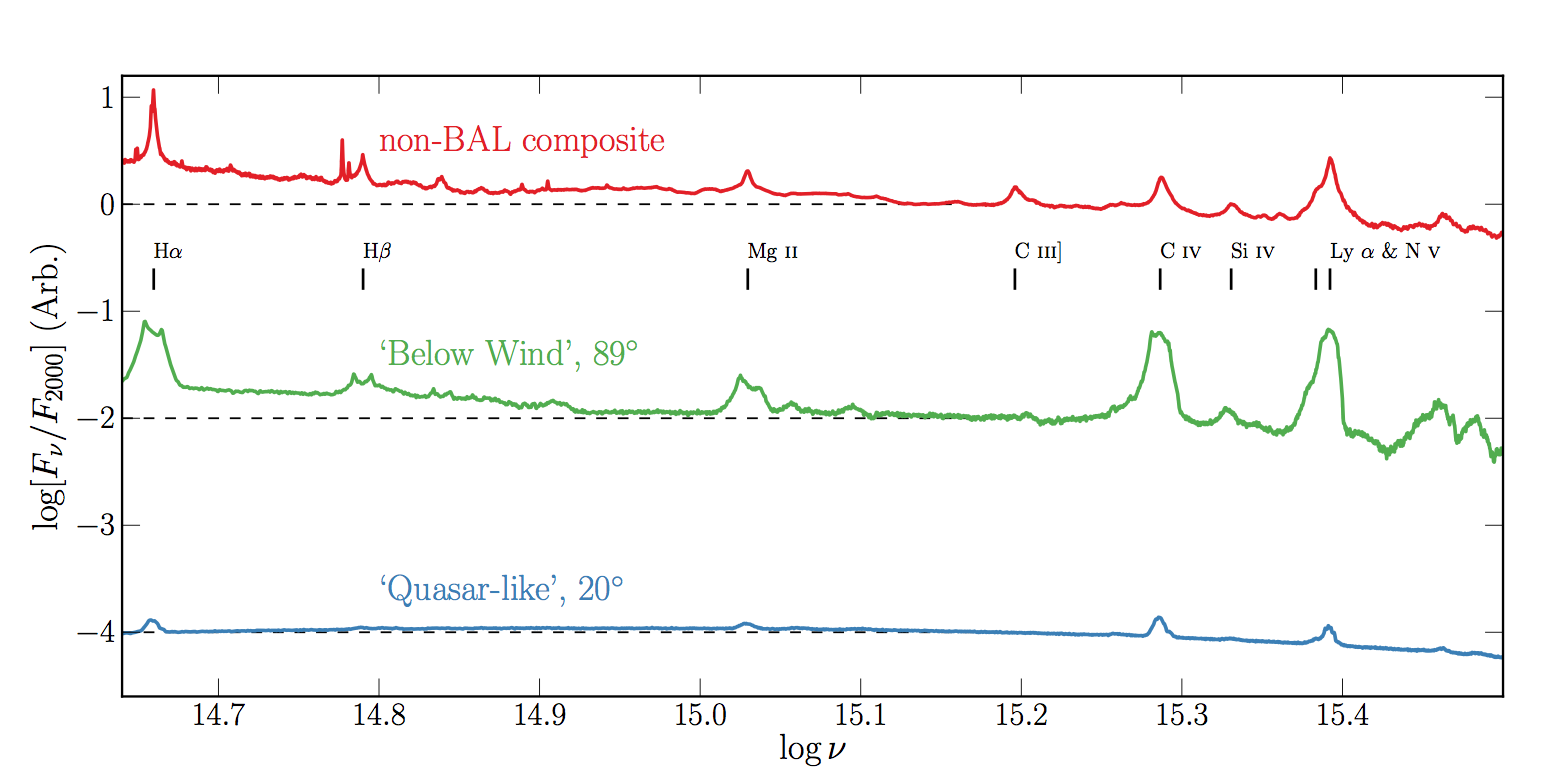
\includegraphics[width=0.9\textheight, angle=270]
{figures/06-agnpaper/fig5.png}
\caption
[Synthetic spectra at two viewing angles compared to the non-BAL SDSS quasar composite.]
{
Synthetic spectra at two viewing angles, 
this time in frequency space and including the optical band,
compared to the non-BAL SDSS quasar composite. The spectra are normalised to the flux at 
$2000$~\AA, then an offset of 2 is applied per spectrum for clarity -- the dotted lines show the zero point of $F_\nu / F_{2000}$ in each case.
}
\label{fig:sed}
\end{figure*}

\noindent
Fig.~\ref{fig:uvspec} shows the synthetic spectrum in the UV from the fiducial model. 
To assess the ability of the synthetic spectra to match real 
quasar spectra, I also show {\sl Sloan Digital Sky Survey} (SDSS) quasar
composites from \cite{reichard2003}, normalised to the flux at 2000~\AA\
for low inclinations. Unfortunately, the wide variety of
line profile shapes and internal trough structure in BALQSOs
tends to `wash out' BAL troughs in composite spectra
to the extent that BALQSO composites do not resemble typical BALQSOs.
Because of this, I instead compare to a {\sl Hubble Space Telescope} 
STIS spectrum of the high BALnicity BALQSO PG0946+301 (Arav et al. 2000),
and an SDSS spectrum of the LoBAL quasar SDSS J162901.63+453406.0,
for the angles of $73^\circ$ and $76^\circ$, respectively. 
A cartoon illustrating how geometric effects determine
the output spectra is shown in Fig.~\ref{fig:sightline}.  

\subsubsection{Broad Absorption Lines (`BALQSO-like' angles)}
\label{sec:balqso_angles}

The UV spectrum is characterised by strong BAL 
profiles at high inclinations ($> 70^\circ$). 
This highlights the first success of the model: 
clumping allows the correct ionization state 
to be maintained in the presence of strong X-rays, 
resulting in large resonance line opacities. 
At the highest inclinations, the 
cooler, low ionization material at the base of the wind
starts to intersect the line of sight. This produces 
multiple absorption lines in species such as \mg,
\al\ and Fe~\textsc{ii}. The potential links to LoBALQSOs and 
FeLoBALQSOs are discussed in section~\ref{sec:lobal}.

The high ionization BAL profiles are often saturated, and the location in velocity space
of the strongest absorption in the profile varies with inclination.
At the lowest inclination BAL sight lines, the strongest absorption occurs at the red edge,
whereas at higher inclinations (and for the strongest BALs)
the trough has a sharp edge at the terminal velocity.
This offers one potential explanation for the wide range of BALQSO absorption
line shapes \citep[see e.g.][]{trump2006,knigge2008,filizak2014}.

The absorption profiles seen in BALQSOs are often non-black, but saturated, 
with flat bases to the absorption troughs \citep{arav1999b,arav1999a}.
This is usually explained either as  partial covering of the continuum
source or by scattered contributions to the BAL troughs, necessarily
from an opacity source not co-spatial with the BAL forming region.
The scattered light explanation is supported by spectropolarimetry results
\citep{lamy2000}. The synthetic spectra do not show non-black, saturated profiles.
Black, saturated troughs are seen at angles $i > 73^\circ$, and the BALs
are non-saturated at lower inclinations. The reasons for this are inherent 
in the construction of the model. 
First, the microclumping assumption does not allow for 
porosity in the wind, meaning that it does not naturally produce
a partial covering absorber. To allow this, an alternative approach
such as {\em macroclumping} would be required \citep[e.g.][]{hamann2008,surlan2012}.
Second, the wind does not have a significant scattering contribution 
along sightlines which do not pass through the BAL region,
meaning that any scattered component to the BAL troughs is absorbed by line opacity.
This suggests that either the scattering cross-section of the wind must
be increased (with higher mass loss rates or covering factors), or 
that an additional source of electron opacity is required, potentially
in a polar direction above the disc. I note the scattering contribution
from plasma in polar regions is significant in some `outflow-from-inflow'
simulations \citep{KP09, simproga2012}.

\subsubsection{Broad Emission Lines (`quasar-like' angles)}

\begin{table}
\centering
\begin{tabular}{p{2cm}p{2cm}p{3cm}}
\hline Property & Synthetic, $20^\circ$ & Observed  (S11) \\ 
\hline \hline
$\log L$[C~\textsc{iv}]  & $44.60$ & $44.42 \pm 0.32$  \\
$\log L$[Mg~\textsc{ii}] & $43.92$ & $43.54 \pm 0.28$  \\
$\log (\nu L_{\nu})_{1350}$  & $46.42$ & $46.01 \pm 0.30$ \\
$\log (\nu L_{\nu})_{3000}$  & $46.18$ & $45.79 \pm 0.30$ \\
\hline
\end{tabular}
\caption
[Some derived spectral properties of the fiducial model compared to observations.]
{
Some derived spectral properties of the fiducial model, at $20^\circ$,
compared to observations. The observed values are taken from the Shen et al. (2011)
SDSS DR7 Quasar catalog, and correspond to mean values with standard deviations in log space
from a subsample with $8.5>\log(M_{BH})<9.5$ and 
$-1.5<\log (L_{\mathrm{bol}}/L_{\mathrm{Edd}}) < 0$,
where the BH mass is a \civ\ virial estimate. 
Units are logarithms of values in erg~s$^{-1}$.
%unless stated.otherwise.
}
\label{line_lums}
\end{table}


Unlike H13, significant collisionally excited line emission now emerges
at low inclinations in the synthetic spectra, particular in the \civ\ and \nv\
lines. Strong \la\ and
weak He~\textsc{ii}~$1640$~\AA\ lines are also observed
as a result of the improved treatment of recombination using macro-atoms. 
In the context of unification, this is a promising result, 
and shows that a biconical wind can produce significant 
emission at `quasar-like' angles. To demonstrate this further,
I show line luminosities and monochromatic continuum luminosities
from the synthetic spectra in table~\ref{line_lums}. These are compared to
mean values from a subsample of the SDSS DR7 quasar catalog \citep{shen2011} 
with BH mass and Eddington fraction estimates similar to the fiducial model values 
(see caption). The spectra do not contain the strong 
C~\textsc{iii}]~1909~\AA\ line seen in the quasar composite spectra, 
but this is due to a limitation of the current treatment of C; semi-forbidden
(intercombination) lines are not included in this modelling.

In Fig.~\ref{fig:sed}, I show an $F_{\nu}$ spectrum with broader waveband coverage
that includes the optical, showing that the synthetic spectra 
also exhibit \ha\ and \hb\ emission. 
In this panel, I include a low inclination and 
also a very high inclination 
spectrum, which looks underneath the wind cone. This model shows 
strong line emission with very similar widths and line ratios to the quasar composites, and
the Balmer lines are double peaked, due to velocity projection effects.  
Such double-peaked lines are seen in so-called `disc emitter' systems 
\citep[e.g.][]{eracleous1994} but not the majority of AGN.     
The line equivalent widths (EWs) increase at high inclination
due to a weakened continuum from wind attenuation, 
disc foreshortening and limb darkening. This effect also 
leads to a redder continuum slope, as seen in quasars, which is
due to Balmer continuum and Balmer and Fe~\textsc{ii} line emission.
This extreme $89^\circ$ viewing angle cannot represent a typical quasar within a unified model,
but does show that a model such as this can naturally reproduce quasar emission lines
if the emissivity of the wind is increased {\em with respect to the disc continuum}.
In addition, it neatly demonstrates how a stratified outflow can naturally
reproduce the range of ionization states seen in quasars. 

Despite a number of successes, 
there are a some properties of the synthetic spectra
that are at odds with the observations. First, the ratios of the 
EW of the \la\ and \mgline\ lines
to the EW of \civline\ are much lower than in the composite spectra. 
Similar problems have also been seen in simpler photoionization models for the 
BLR \citep{netzer1990}.
It may be that a larger region of very dense ($n_e\sim10^{10}$cm$^{-3}$) 
material is needed, which could correspond to a disc atmosphere or 
`transition region' 
\citep[see e.g.][]{MCGV95,knigge1998}. \nocite{knigge1998} 
While modest changes to geometry may permit this, the initial grid search 
did not find a parameter space in which the \la\ or \mg\ EWs
were significantly higher (see section~\ref{sec:param_sens}). 
Second, EWs increase with inclination 
(see Fig.~\ref{fig:uvspec} and Fig.~\ref{fig:sed}; also Fig.~\ref{fig:lobal}).
This is discussed further in section~\ref{sec:ew_in_model}.

\subsection{X-ray Properties}
\label{sec:xray}


\begin{figure*}
\centering
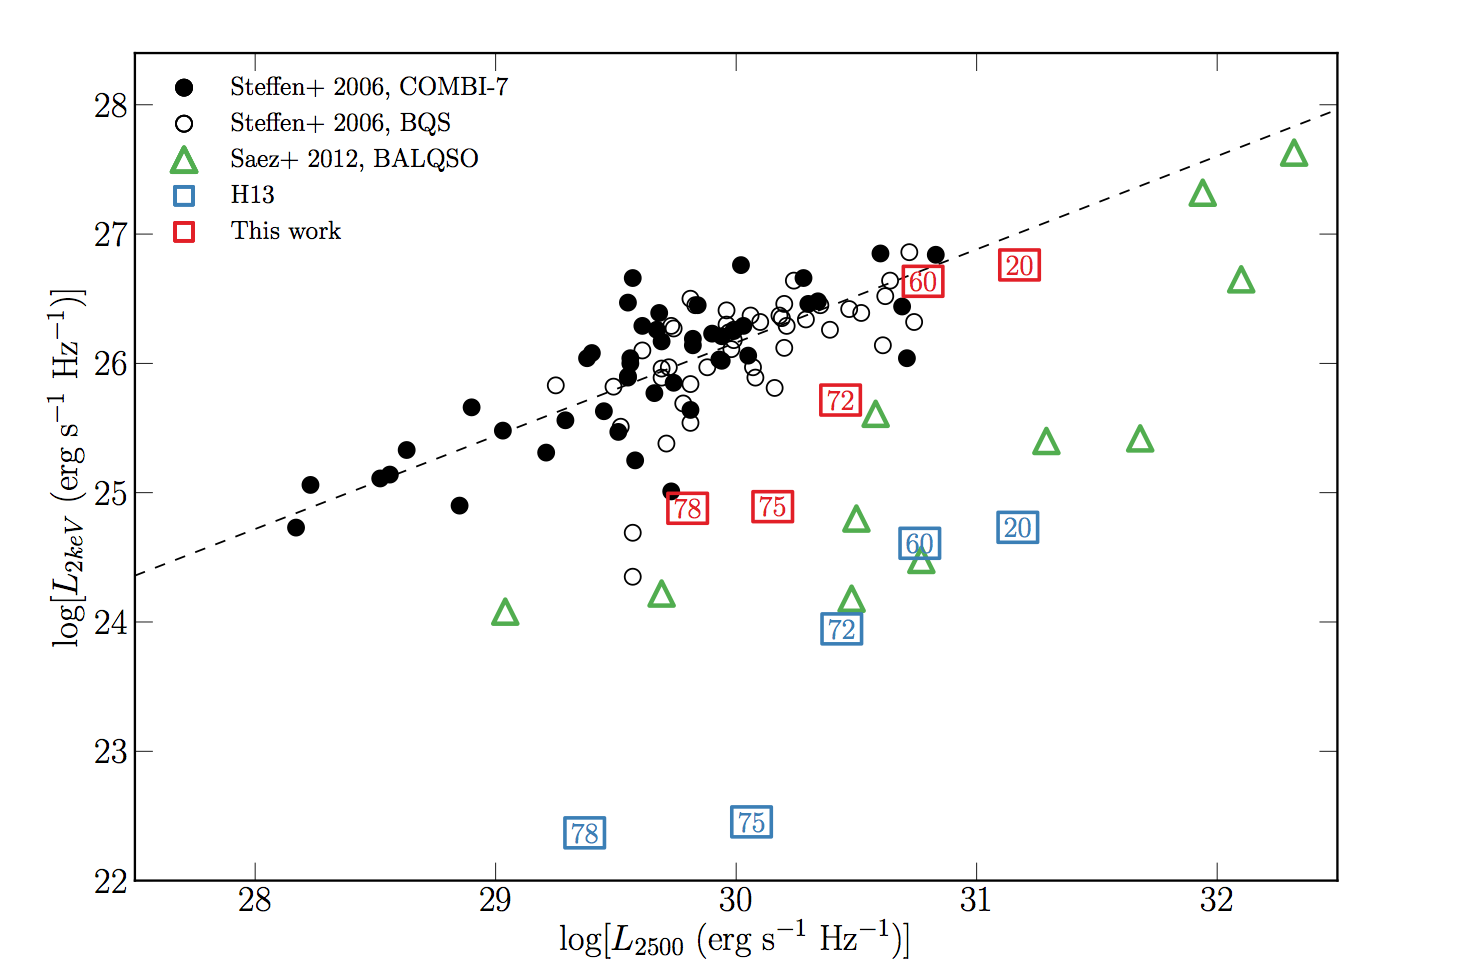
\includegraphics[width=1.0\textwidth]{figures/06-agnpaper/fig6.png}
\caption
[X-ray properties of the clumped quasar model compared to H13 and samples
from the literature.]
{
X-ray ($2$~keV) luminosity of the clumped model (red squares) 
and the H13 model (blue squares), plotted against monochromatic luminosity 
at 2500~\AA. The points are labeled according to inclination; angles
$>70^\circ$ correspond to BALs in this scheme (see Fig.~\ref{fig:sightline}).
Also plotted are masurements from 
the COMBI-7 AGN and the BQS samples (Steffen et al. 2006) and the Saez et al. (2012) 
sample of BALQSOs. The dotted line shows the best fit relation for non-BALQSOs 
from Steffen et al. (2006).
}
\label{fig:xray}
\end{figure*}

The main motivation for adding clumping to the model was
to avoid over-ionization of the wind in the presence of strong X-rays. 
Having verified that strong BALs appear in the synthetic spectra,
it is also important to assess whether the X-ray properties of this
fiducial model agree well with quasar and BALQSO samples for the relevant
inclinations.

Fig.~\ref{fig:xray} shows the emergent
monochromatic luminosity ($L_\nu$) at 2~keV and 
plotted against $L_\nu$ at $2500$~\AA\ 
for a number of different viewing angles in the model.
The monochromatic luminosities are calculated from the synthetic spectra and thus include
the effects of wind reprocessing and attenuation. In addition to model outputs,
I also show the BALQSO sample of Saez et al. (2012) and luminous AGN and quasar
samples from Steffen et al. (2006). The best fit relation from Steffen et al. (2006) 
is also shown. For low inclination, `quasar-like' viewing angles,
the model properties are in excellent agreement with AGN samples. The slight gradient from $20^\circ$ to
$60^\circ$ in the models is caused by a combination of disc foreshortening and limb-darkening 
(resulting in a lower $L_{2500}$ for higher inclinations), and the fact that the disk 
is opaque, and thus the X-ray source subtends a smaller solid angle at high inclinations
(resulting in a lower $L_{2keV}$ for higher inclinations). 


The high inclination, `BALQSO-like' viewing angles show moderate agreement with the data,
and are X-ray weak due to bound-free absorption and electron scattering in the wind.
Typically, BALQSOs show strong X-ray absorption with columns 
of $N_H\sim10^{23}~\rm{cm^{-2}}$ 
\citep{green1996,mathur2000,green2001,grupemathur2003}.
This is often cited as evidence that the BAL outflow is shielded from
the X-ray source, especially as sources with strong X-ray absorption tend
to exhibit deep BAL troughs and high outflow velocities 
\citep{brandt2000,laorbrandt2002,gallagher2006}.
These results imply that the clumpy BAL outflow
itself can be responsible for the strong X-ray absorption, 
and supports the suggestion of \cite{hamann2013} that 
geometric effects explain the weaker X-ray absorption in mini-BALs 
compared to BALQSOs.

\subsection{LoBALs and Ionization Stratification}
\label{sec:lobal}
\begin{figure*}
\centering
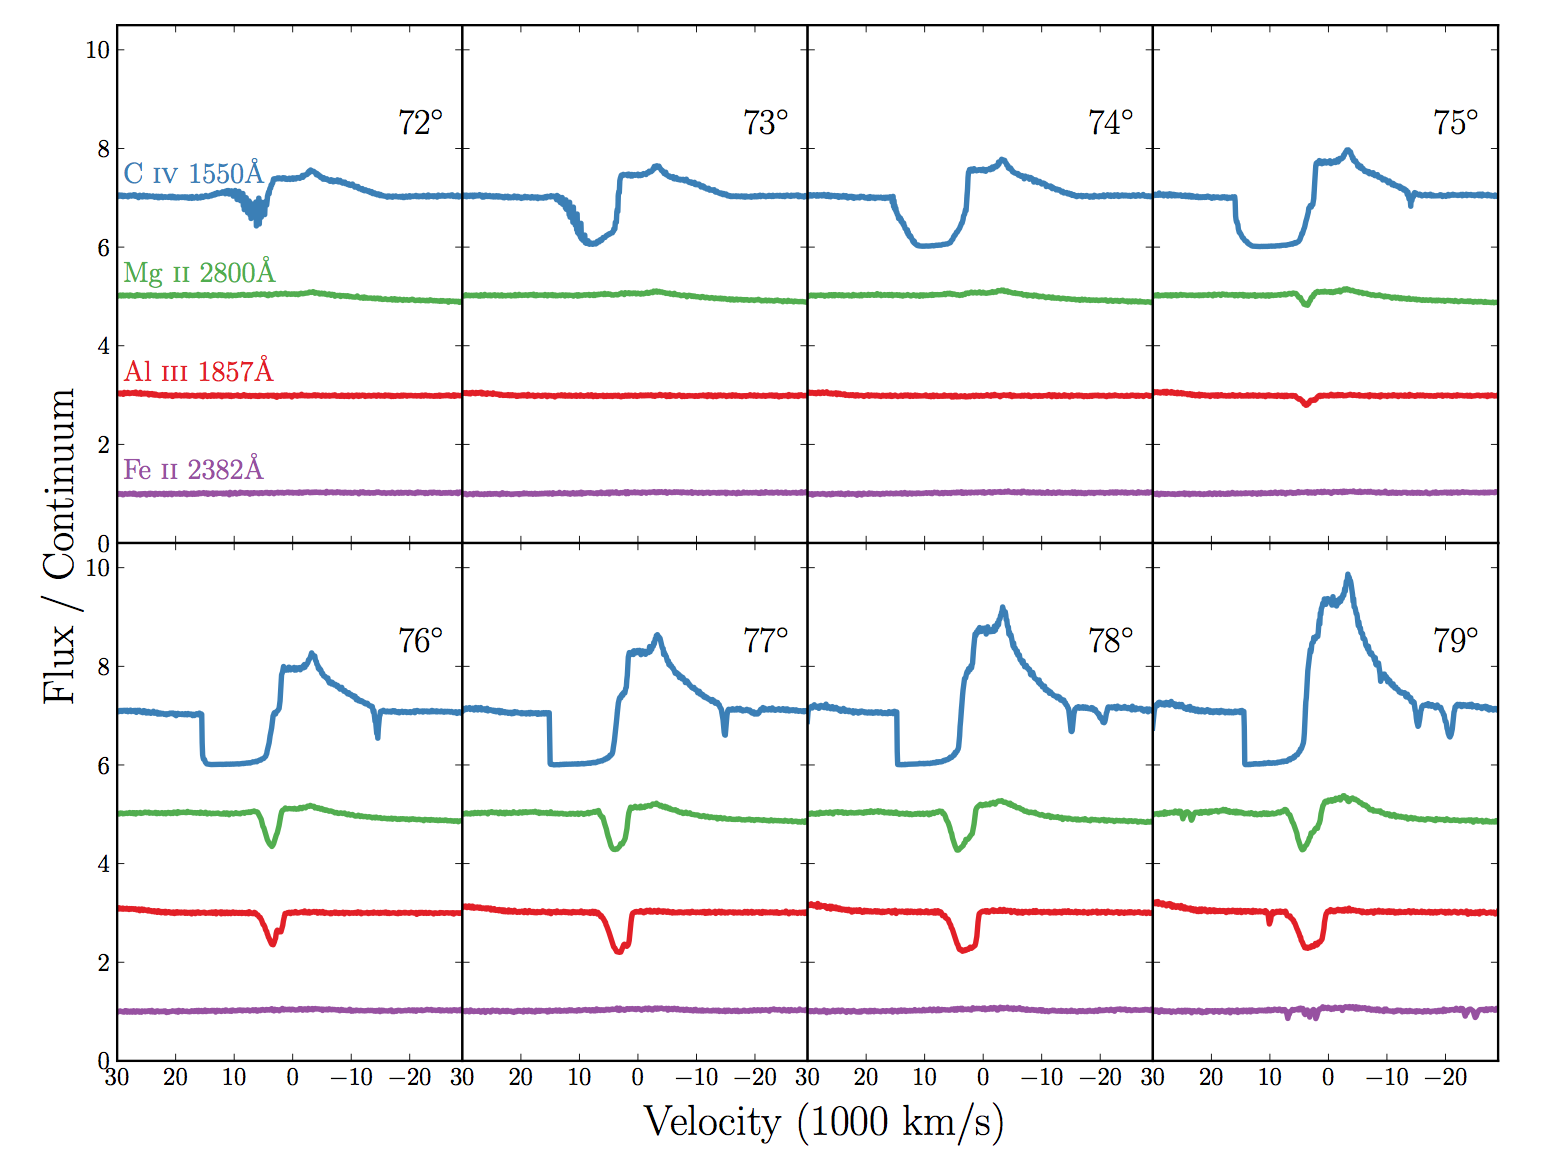
\includegraphics[width=1.0\textwidth]{figures/06-agnpaper/fig7.png}
\caption
[\civ , \mg , \al\ and Fe~\textsc{ii} line profiles for wind viewing angles.]
{
\civ , \mg , \al\ and Fe~\textsc{ii} line profiles for viewing angles
from $72-79^\circ$. The profiles are plotted relative to the local
continuum with an offset applied for clarity. Lower ionization
profiles appear at a subset of high inclinations, compared
to the ubiquitous \civ\ profile.
}
\label{fig:lobal}
\end{figure*}


At high inclinations, the synthetic spectra exhibit 
blue-shifted BALs in \al\ and \mg --
the absorption lines seen in LoBALQSOs -- 
and even show absorption in Fe~\textsc{ii}
at the highest inclinations. Line profiles in velocity space 
for \civ, \al\ and \mg, are shown in Fig.~\ref{fig:lobal} for a range
of BALQSO viewing angles. Ionization stratification
of the wind causes lower ionization material to have a 
smaller covering factor, 
as demonstrated by figures~\ref{fig:wind} and \ref{fig:lobal}.
This confirms the behaviour expected from a unification model such as Elvis (2000). 
LoBALs are only present at viewing angles close to edge-on ($i>75^\circ$),
as predicted by polarisation results \citep{brotherton1997}.
As observed in a BALQSO sample by \cite{filizak2014}, 
the model BAL troughs are wider and deeper when low ionization 
absorption features are present,
and high ionization lines have higher blue-edge velocities than the 
low ionization species.
There is also a correlation between the strength of LoBAL features
and the amount of continuum attenuation at that sightline, particularly
blueward of the Lyman edge as the low ionization base 
intersects the line-of-sight. 
A model such as this therefore predicts that LoBALQSOs and FeLoBALQSOs 
have stronger Lyman edge absorption and 
are more Compton-thick than HiBALQSOs and Type 1 quasars.
An edge-on scenario also offers a potential explanation for the rarity of LoBAL and
FeLoBAL quasars, due to a foreshortened and attenuated continuum, 
although BAL fraction inferences are fraught with complex selection 
effects \citep{goodrich1997,krolikvoit1998}.


\section{Discussion}
\label{sec:qso_discuss}

\subsection{Parameter Sensitivity}
\label{sec:param_sens}

\begin{figure*}
\centering
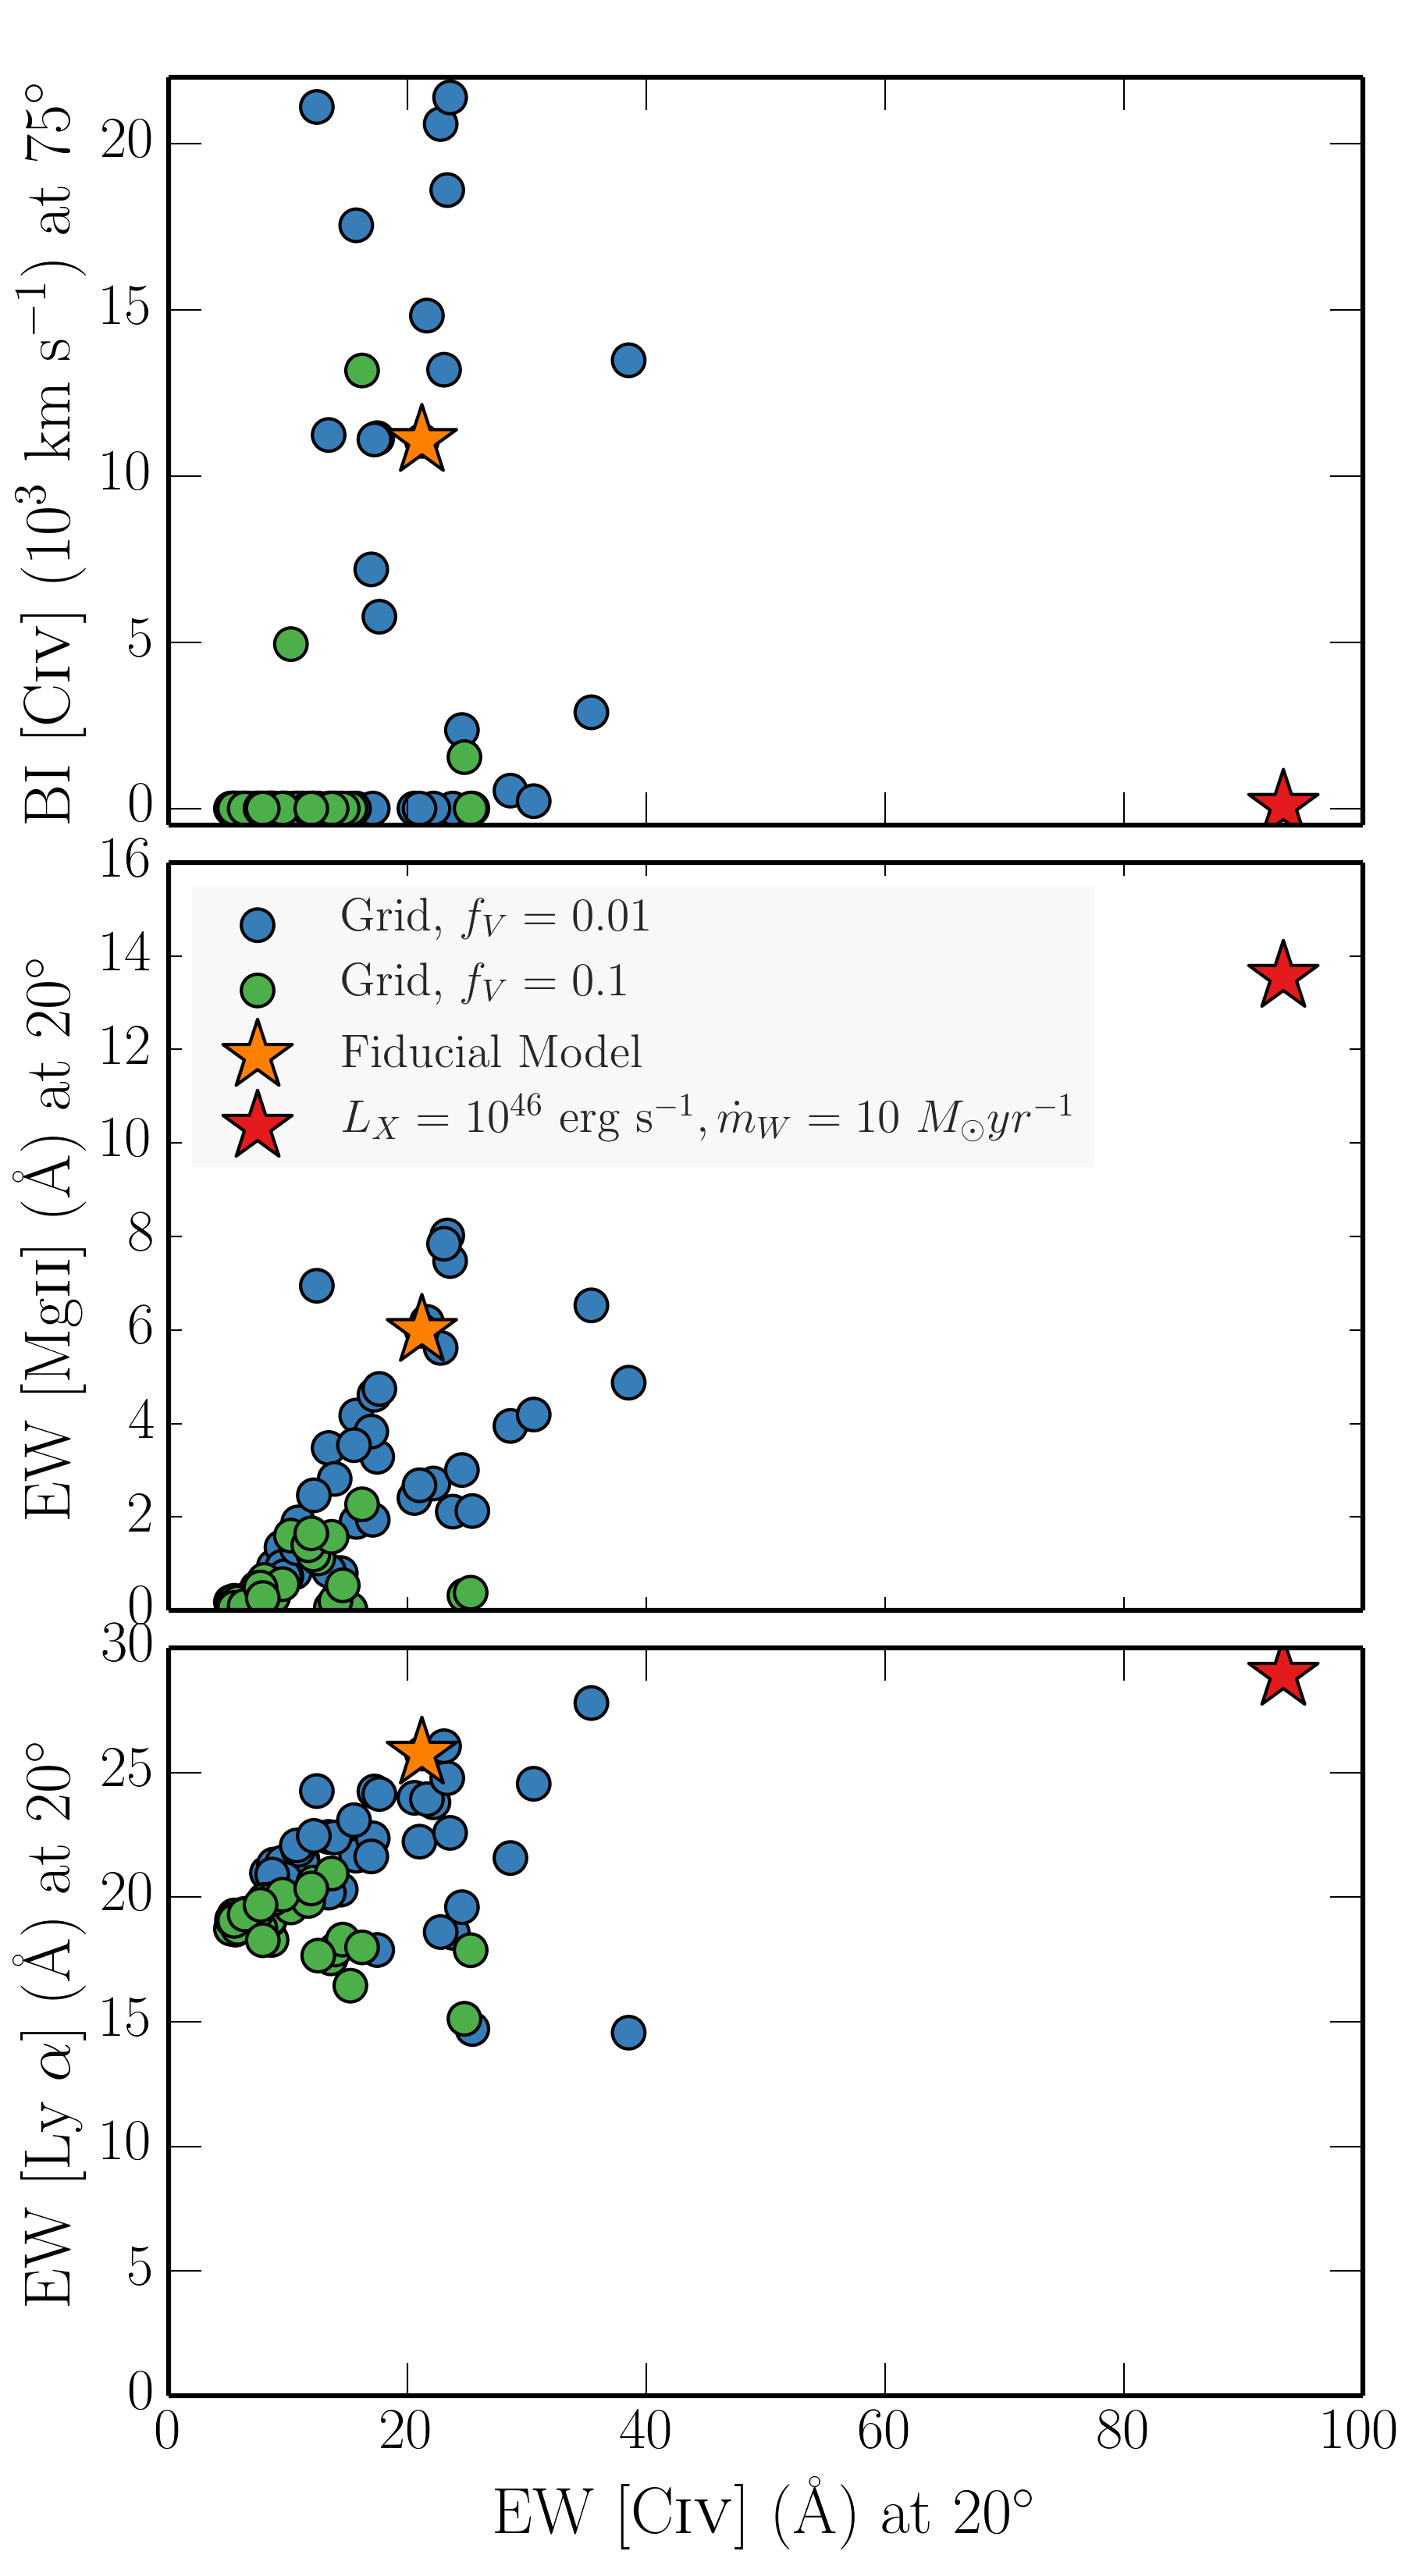
\includegraphics[width=0.8\textwidth]
{figures/06-agnpaper/thesis_c4_grid.png}
\caption
[Equivalent widths and BALnicities of some important lines for the quasar wind grid.]
{
The EW of the \civ~$1550$~\AA\ line at $20^\circ$ plotted against a) the 
$BI$ of \civ~$1550$~\AA\ at $75^\circ$, b) the EW of the \mg~$2800$~\AA\ line 
at $20^\circ$ and c) the EW of \la\ at $20^\circ$. The circles correspond 
to the simulation grid for two different values of $f_V$, and the fiducial 
model is marked with an orange star. 
I also show a higher X-ray luminosity model and a higher mass loss rate
with a red star.
}
\label{fig:grid}
\end{figure*}

Having selected an individual fiducial model from the simulation grid, it is important
to briefly explore how specialised this model is, and how small parameter
changes can affect the synthetic spectra. Fig.~\ref{fig:grid}
shows the EW of \la, \civline\ and \mgline\ 
for a representative low inclination, and the $BI$ for a 
representative high inclination, as produced by the models in the simulation
grid. A few conclusions can be drawn from this plot straight away. 
First, almost all the models with 
$f_V=0.1$ are over-ionized and 
fail to produce strong \civ\ BALs or emission lines. Second,  
it is difficult to significantly increase line emission while
keeping the luminosity and mass-loss rate of the system fixed. 
I show an additional point on Fig.~\ref{fig:grid} corresponding to a 
model with an order of
magnitude higher X-ray luminosity and double the mass loss rate. As expected, 
this results in far higher line EWs, but fails to produce BALs, because
the collisionally excited emission swamps the BAL profile. In addition,
this model would lie well above the expected $L_{2kev}-L_{2500}$ 
relation in Fig.~\ref{fig:xray}. Such a high X-ray luminosity could therefore 
not be the cause of the strong line emission seen in {\em all} Type 1 quasars.

The parameter search presented here is by no means exhaustive, and
conclusions may be limited by the specific parameterisation of the outflow 
kinematics used. Nevertheless, I suggest that the angular distribution
of both the line and continuum emission is perhaps the crucial 
aspect to understand. With this in mind, obtaining reliable orientation 
indicators appears to be a crucial observational task if we are to
further our understanding of BAL outflows and their connection, or lack thereof, to the 
broad line region. 

\subsection{Inclination Trends: FWHM and EW}
\label{sec:ew_in_model}

Broad line EWs increase with inclination in the fiducial model.
This trend means that even though models with
significantly denser and more strongly irradiated winds
can match the line EWs fairly well at low inclinations, they also
produce overly strong red wings to the BAL P-Cygni profiles at high inclinations.
This trend with inclination is directly related to limb-darkening 
and foreshortening of the model continuum. 
However, it appears to contradict observations, which show remarkably uniform emission
line properties in quasars and BALQSOs \citep{weymann1991,dipompeo2012b}. 

In order to quantitatively assess how emission lines change with 
inclination when blue-shifted absorption 
may affect the line profile, I define the `red wing equivalent width' (EW$_{RW}$) as
\begin{equation}
\mathrm{EW}_{RW} = \int_{\lambda_0}^{\lambda^\prime} \left( 1 - \frac{F_\lambda}{F_0} \right) d\lambda,
\label{rwew}
\end{equation}
where $F_0$ is the continuum flux, and the integral is calculated from $\lambda_0$, line centre,
to a wavelength $\lambda^\prime$ where the flux has returned to the continuum level.
This quantity is shown as a function of inclination in Fig.~\ref{fig:ew_in_model} for the \civ\ UV line.
I also show $1/2$ the EW value, together with the standard deviation, from \cite{dipompeo2012b}.

\begin{figure*}
\centering
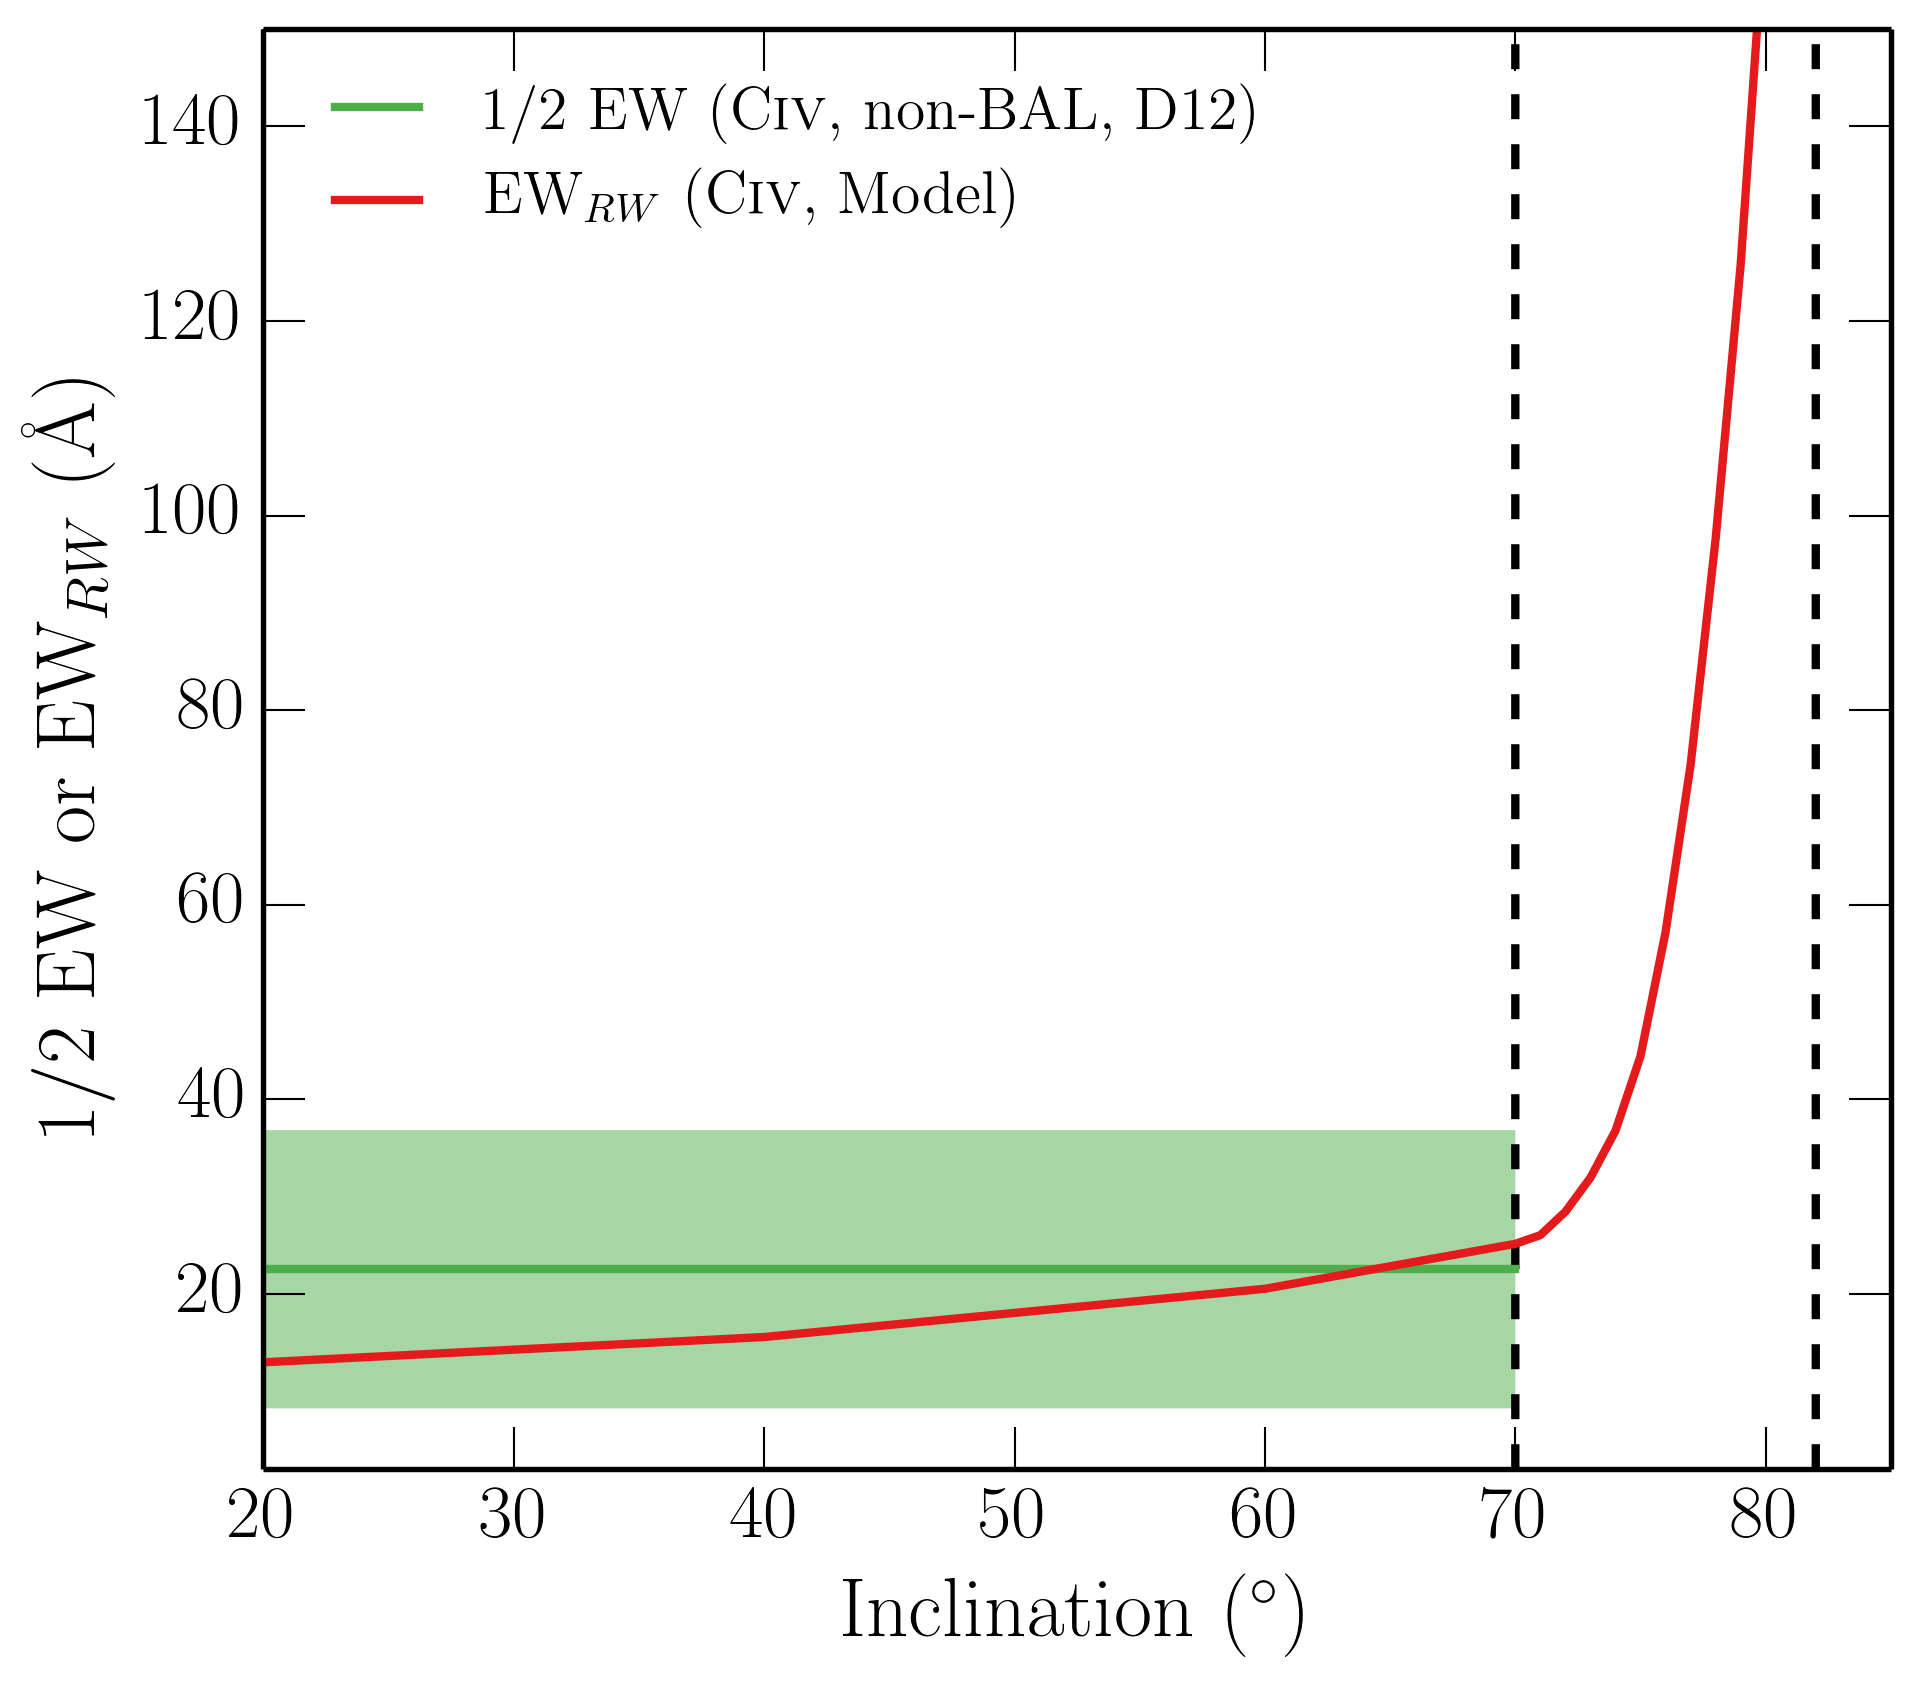
\includegraphics[width=0.8\textwidth]{figures/ewpaper/ew.png}
\caption
[EW$_{RW}$ as a function of inclination in the fiducial model.]
{
EW$_{RW}$ as a function of inclination in the fiducial model, compared
to 1/2 EW from the quasar sample of Di Pompeo et al. (2012; D12). The shaded region
corresponds to the standard deviation of the D12 sample.
}
\label{fig:ew_in_model}
\end{figure*}

The variation of EW with inclination is significantly 
larger than the variation across the quasar population.
The angular distribution of the disc 
continuum and line emission is clearly crucially important in 
determining the emergent broad line EWs, as suggested by, e.g., 
the analysis of \cite{risaliti2011}. 
I shall explore this question further in chapter 6.  

\subsubsection{FWHM and Black Hole Mass Estimates}
\label{sec:model_fwhm}
In a recent study, \cite[hereafter Y16]{yong2016} used the SV93 wind prescription to
assess the variation of full-width at half-maximum (FWHM) of 
\hb\ (and resultant BH mass estimates)
with inclination in a disc wind model. 
Although their model is fairly simple -- 
it does not include, for example, full radiative transfer or ionization physics --
this analysis still gives interesting insights into how emission lines
from a disc wind might bias BH mass estimates.

If the BLR gas is virialised, as often assumed, then the black hole mass
is related to the velocity dispersion, $\Delta v$, of the gas by
\begin{equation}
M_{BH} = f \frac{\Delta v^2 R_{BLR}}{G},
\end{equation}
where $R_{BLR}$ is some appropriate emissivity-weighted radius and is often 
either assumed, estimated from ionization arguments or calculated from reverberation
mapping. When using the FWHM of a broad emission line to estimate the velocity disperson the above
equation can be rewritten as
\begin{equation}
M_{BH} = f_{FWHM}~\left[c~\frac{(FWHM)}{\lambda_0}\right]^2~\frac{R_{BLR}}{G},
\end{equation}
where $\lambda_0$ is the central wavelength of the line in question
and the FWHM is in the same wavelength units.

In our benchmark disc wind model, the BH mass is known, and determines
the escape velocities and rotational motions of the outflow. Thus, 
using a typical radius for line formation in the model, it is trivial to 
estimate $f_{FWHM}$ for each viewing angle. Fig.~\ref{fig:FWHM}
shows $f_{FWHM}$ as a function of inclination for the 
\ha\ emission line in the fiducial model, assuming $R_{BLR}=10^{17}$~cm. 
The results are compared to predicted values for five Seyfert I galaxies
from dynamical modelling \citep[][hereafter P14]{pancoast2014b}, 
and the Y16 predictions. Y16 designed two models 
in order to mimic those proposed by MCGV95 and \cite{elvis2000}, 
whose models are described in section~\ref{sec:wind_models}. 
Note that I have used FWHM of \ha\ rather than \hb\ due to the
low \hb\ luminosity at some viewing angles. Nevertheless,
this value should trace $f_{FWHM}$ from \hb\ fairly well.

\begin{figure}
\centering
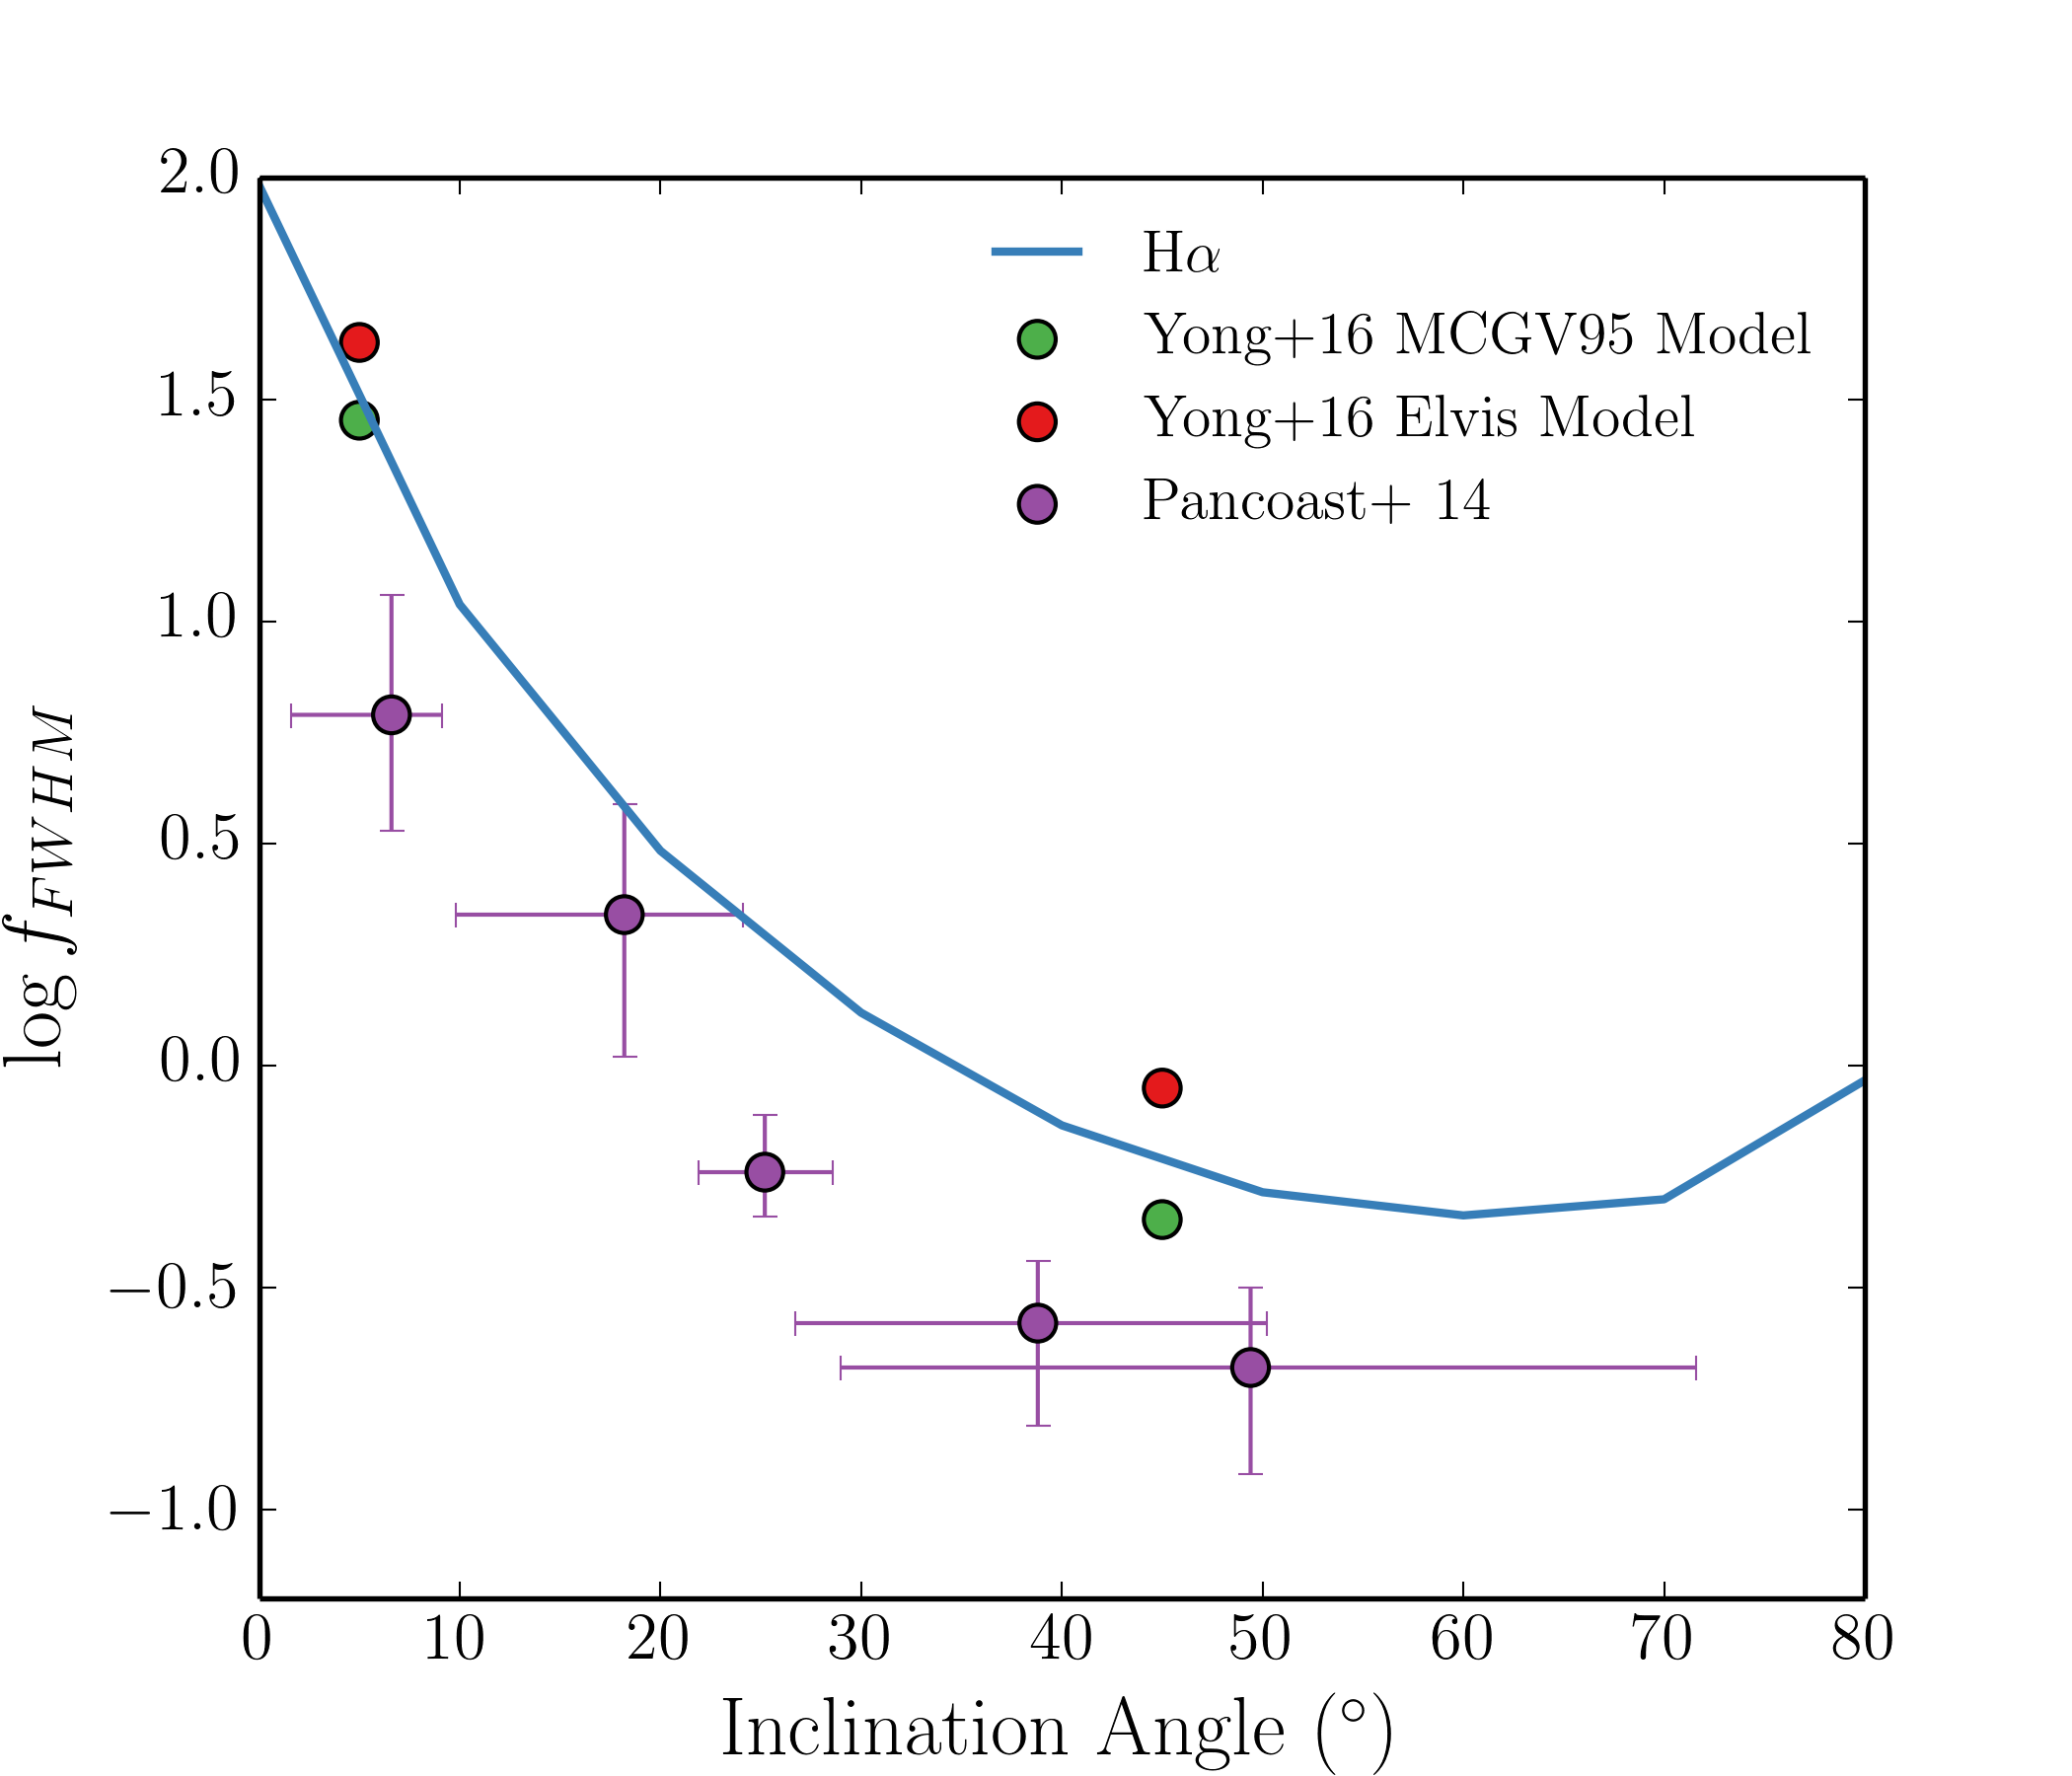
\includegraphics[width=0.8\textwidth]{figures/06-agnpaper/f_factor.png}
\caption
[$f_{FWHM}$ as a function of inclination from the fiducial model.]
{
$f_{FWHM}$ as a function of inclination from the fiducial model
for three different lines. The Yong et al. (2016) 
predictions from two models, and the Pancoast et al. (2014) modelling results
for five Seyfert I galaxies are also shown.
}
\label{fig:FWHM}
\end{figure}

At `quasar-like' angles ($0^\circ-60^\circ$), the values from the model presented here 
agree fairly well with the predictions
of Y16 from their simpler analysis, suggesting that,
at least in this specific set-up, 
radiative transfer and ionization has a minimal role in determining
the emergent FWHM at those angles. Instead, at low inclinations 
the effect is dominated by velocity projection
effects. At inclinations looking into the wind radiative transfer
and shielding effects become important, and the FWHM can actually
decrease. The similarity in the shape of the curve to the P14 results suggest 
that the behaviour of FWHM is somewhat degenerate with the BLR
geometry. P14 found a thick disc model for the BLR best reproduced
the observations, but these results suggest that a wind model can mimic 
the behaviour of a disc-shaped BLR. Overall, the strong inclination dependence
of $f_{FWHM}$ strengthens the argument that viewing angle can introduce
significant uncertainty into virial mass estimates, and that individual
values for $f_{FWHM}$ should really be used for different objects
\citep[e.g.][]{decarli2008,kollatschny2011,pancoast2014a,pancoast2014b,shenho2014,brotherton2015,yong2016}.
% The reason for the significantly lower values for \mgii\ is that
% it is actually formed well inside $R_{BLR}=10^{17}$~cm, highlighting
% the dangers of using a single BLR radius for BH mass estimates
% from different lines.


%%%%%%%%%%%%%%%%%%%%%%%%%%%%%%%%%%%%%%%%%%%%%%%%%

% SUMMARY

%%%%%%%%%%%%%%%%%%%%%%%%%%%%%%%%%%%%%%%%%%%%%%%%%

\section{Summary And Conclusions}
\label{sec:qso_conclusions}
I have carried out MCRT simulations using a simple
prescription for a biconical disc wind, with
the aim of expanding on the work of H13. To do this, two main
improvements were necessary: First, I included a simple treatment of 
clumping, and second, 
the modelling of recombination lines was improved by treating H and He as
`macro-atoms'. 
Having selected a fiducial model from an initial simulation grid,
I assessed the viability of such a model for geometric 
unification of quasars, and found the following main points:
\begin{enumerate}
\item Clumping moderates the ionization state
sufficiently to allow for the 
formation of strong UV BALs while agreeing well with the X-ray
properties of luminous AGN and quasars. 
\smallskip
\item A clumpy outflow model naturally 
reproduces the range of ionization states
expected in quasars, due to its stratified density
and temperature structure. 
LoBAL line profiles are seen at a subset of viewing angles, and Fe~\textsc{ii}
absorption is seen at particularly high inclinations. 
\smallskip
\item The synthetic spectra show a strong \la\ line and weak He~\textsc{ii}~$1640$~\AA\ emisson line,
as a result of the improved treatment of recombination using macro-atoms. 
Balmer emission lines and a Balmer recombination continuum are also
seen in the optical spectrum, but this
is only really significant at high inclination where 
the continuum is suppressed.  
\smallskip
\item The higher X-ray luminosity causes a significant 
increase in the strength of the collisionally excited emission
lines produced by the model. 
However, the equivalent-width ratios of the emission lines do not match
observations, suggesting that a greater volume of dense ($n_e\sim10^{10}$~cm$^{-3}$)
material may be required.
\smallskip
\item The line EWs in the synthetic spectra increase with inclination.
BAL and non-BAL quasar composites have comparable EWs, so the fiducial model
fails to reproduce this behaviour.
 If the BLR emits fairly isotropically then for a 
foreshortened, limb-darkened accretion disc 
it is not possible to achieve line ratios at low inclinations 
that are comparable to those at high inclinations. 
I suggest that understanding the angular distribution of 
line and continuum emission is a crucial question for theoretical models.
\smallskip
\item There is also a strong dependence on inclination in the FWHM of
\ha, as found in numerous other studies. The results add to the growing evidence
that inclination introduces large uncertainties into virial 
BH mass estimates, and suggest that disc wind models might produce similar inclination-dependent
behaviour in $f_{FWHM}$ to disc-shaped BLR models.
% Furthermore, this is conclusion is independent of the assumed 
% BLR geometry and size.
\end{enumerate}
This work confirms a number of expected outcomes from a geometric unification 
model, and suggests that a simple biconical geometry such as this can come close to 
explaining much of the  phenomenology of quasars. However, these conclusions pose 
some challenges to a picture in which BALQSOs are
explained by an {\em equatorial} wind rising from a classical thin disc, and suggest 
the angular distribution of emission is important to understand if this 
geometry is to be refuted or confirmed. I suggest that obtaining reliable 
observational orientation indicators and 
exploring a wider parameter space of outflow geometries in simulations
are obvious avenues for future work.